\section{Implementation of s-channel models}

There are several matrix element implementations of the
DM production through spin-0 and spin-1 mediators.

For a spin-1 mediator, the implementation in POWHEG generates
DM pair production with 1 parton at next-to-leading order (NLO), whilst MADGRAPH and MCFM are at leading order (LO). As shown in POWHEG Ref.\,\cite{Haisch:2013ata}, including NLO corrections result in an enhancement in the cross section as compared to LO and though this is not significant, it does lead to a substantial reduction in the dependence on the choice of the renormalization and factorization scale and hence the theoretical uncertainty on the signal prediction. 
Since NLO calculations are available for the process in POWHEG, we recommend to proceed with POWHEG as the generator of choice. 

For a spin-0 mediator, the top-quark loop is the most important
consideration.
The matrix element implementation of the s-channel spin-0 mediated DM production is available in POWHEG with the full top-loop calculation at LO\,\cite{Haisch:2015ioa}.
The POWHEG implementation includes the finite
top quark mass dependence for DM pair production with 1 parton at LO.
For consistency with the spin-1 generation, we recommend using POWHEG
for this case as well.


Here, we document some specific settings for the Dark Matter models
needed to run the POWHEG generation:
\begin{itemize}
\item The POWHEG implementation allows to generate a single sample that provides sufficient statistics in all signal regions. %by optimizing the following two parameters:
%\begin{itemize}
POWHEG generates weighted events and the \verb+bornsuppfact+ parameter is used to set the event suppression factor according to
\begin{equation}
F(k_{\rm{T}})=\frac{k_{\rm{T}}^2}{k_{\rm{T}}^2+\texttt{bornsuppfact}^2} \;.
\end{equation}
In this way, the events at, for instance low $\MET$, are suppressed and receive higher event weights which ensures higher statistics at high $\MET$. We recommend to set \verb+bornsuppfact+ to 1000.
\item The \verb+bornktmin+ parameter allows to suppress the low $\MET$ region even further by starting the generation at a certain value of $k_{\rm{T}}$. It is recommended to set this parameter  to half the lower analysis $\MET$ cut, for the event selection used in the CMS/ATLAS monojet analyses for instance the proposed value for \verb+bornktmin+ is 150. However, this parameter should be set keeping in mind the event selection of all the analyses that will use these signal samples and hence a threshold lower than 150 may be required. 
%\end{itemize}

\item Set \verb+runningwidth+ to 0.
\item Set \verb+mass_low+ and \verb+mass_high+ to -1.
\item The minimal values for \verb+ncall1+, \verb+itmx1+, \verb+ncall2+, \verb+itmx2+ are 250000, 5, 1000000, 5 for the DMV model, respectively. In order to increase speed, set \verb+foldsci+ and \verb+foldy+ to 2 and keep \verb+foldphi+ at 1. 
\item The minimal values for \verb+ncall1+, \verb+itmx1+, \verb+ncall2+, \verb+itmx2+ are 100000, 5, 100000, 5 for the DMS\_tloop model, respectively.
\item Allow negative weights for the DMV model by setting \verb+withnegweights+ to 1.
\item Since the DMS\_tloop model is a leading order process, set \verb+LOevents+ and \verb+bornonly+ are set to 1 internally.
\item Automatic calculation of systematic uncertainties associated with the choice of hard scale and PDFs.
\end{itemize}
{\bf [Comment on proper PDF sets to use, concerns about sea quark PDF in b-initiated diagrams (perhaps the latter belongs in the b-flavored DM section]}


\section{CKKW parton matching implementation}
\label{sec:monojet_parton_match}

The parton matching techniques are implemented in the mono-jet like MC generation in order to avoid double counting the partons from matrix elements and parton showering. The CKKW matching is better developed and preferred~\cite{Alwall:1405.0301}~\cite{Alwall:0706.2569}. As the illustration sample, the EFT D5 samples are generated with \texttt{MadGraph5\_aMC@NLO} version 2.2.2. The technical implementations are shown as below.

On the generator side, i.e., \texttt{MadGraph5\_aMC@NLO}:
\begin{itemize}
\item \texttt{ickkw = 0}
\item \texttt{ktdurham = }matching scale
\item \texttt{dparameter = 0.4}
\item \texttt{dokt = T}
\item \texttt{ptj=20}
\item \texttt{drjj=0}
\item \texttt{mmjj=0}
\item \texttt{ptj1min=0}
\end{itemize}
On the parton showering side, i.e., \texttt{Pythia 8}:
\begin{itemize}
\item \texttt{Merging:ktType           = 1}
\item \texttt{Merging:TMS              = }matching scale
\item \texttt{1000022:all = chi chi~ 2 0 0 30.0 0.0 0.0 0.0 0.0}
\item \texttt{1000022:isVisible = false}
\item \texttt{Merging:doKTMerging      = on}
\item \texttt{Merging:Process          = pp>{chi,1000022}{chi~,-1000022}}
\item \texttt{Merging:nJetMax          = 2}
\end{itemize}
The matching scales should be the same for the generation and parton showering. In \texttt{MadGraph5\_aMC@NLO}, the particle data group ID \texttt{1000022} is used for weakly interacting dark matter candidates, which should be informed to \texttt{Pythia 8}. 

In this test we are generating the process with up to two parton emissions, so the command \texttt{Merging:nJetMax = 2} is applied to \texttt{Pythia 8}. The different parton emission cases are generated separately:
\begin{itemize}
\item \texttt{p p > chi chi~}
\item \texttt{p p > chi chi~ j}
\item \texttt{p p > chi chi~ j j}
\end{itemize}
Two matching scales are tested at 30 and 80 GeV. The differential jet rates are shown in Fig. \ref{fig:CKKW_D5_30} for matching scale 30 GeV and Fig. \ref{fig:CKKW_D5_80} for 80 GeV. The 80 GeV matching scale gives smoother distribution, which is desired to avoid artifical effect due to parton matching. There will be a small tink around the matching scale for both cases.

\begin{figure}[h!]
	\centering  
	\subfloat[$1\rightarrow2$ parton process]{%
		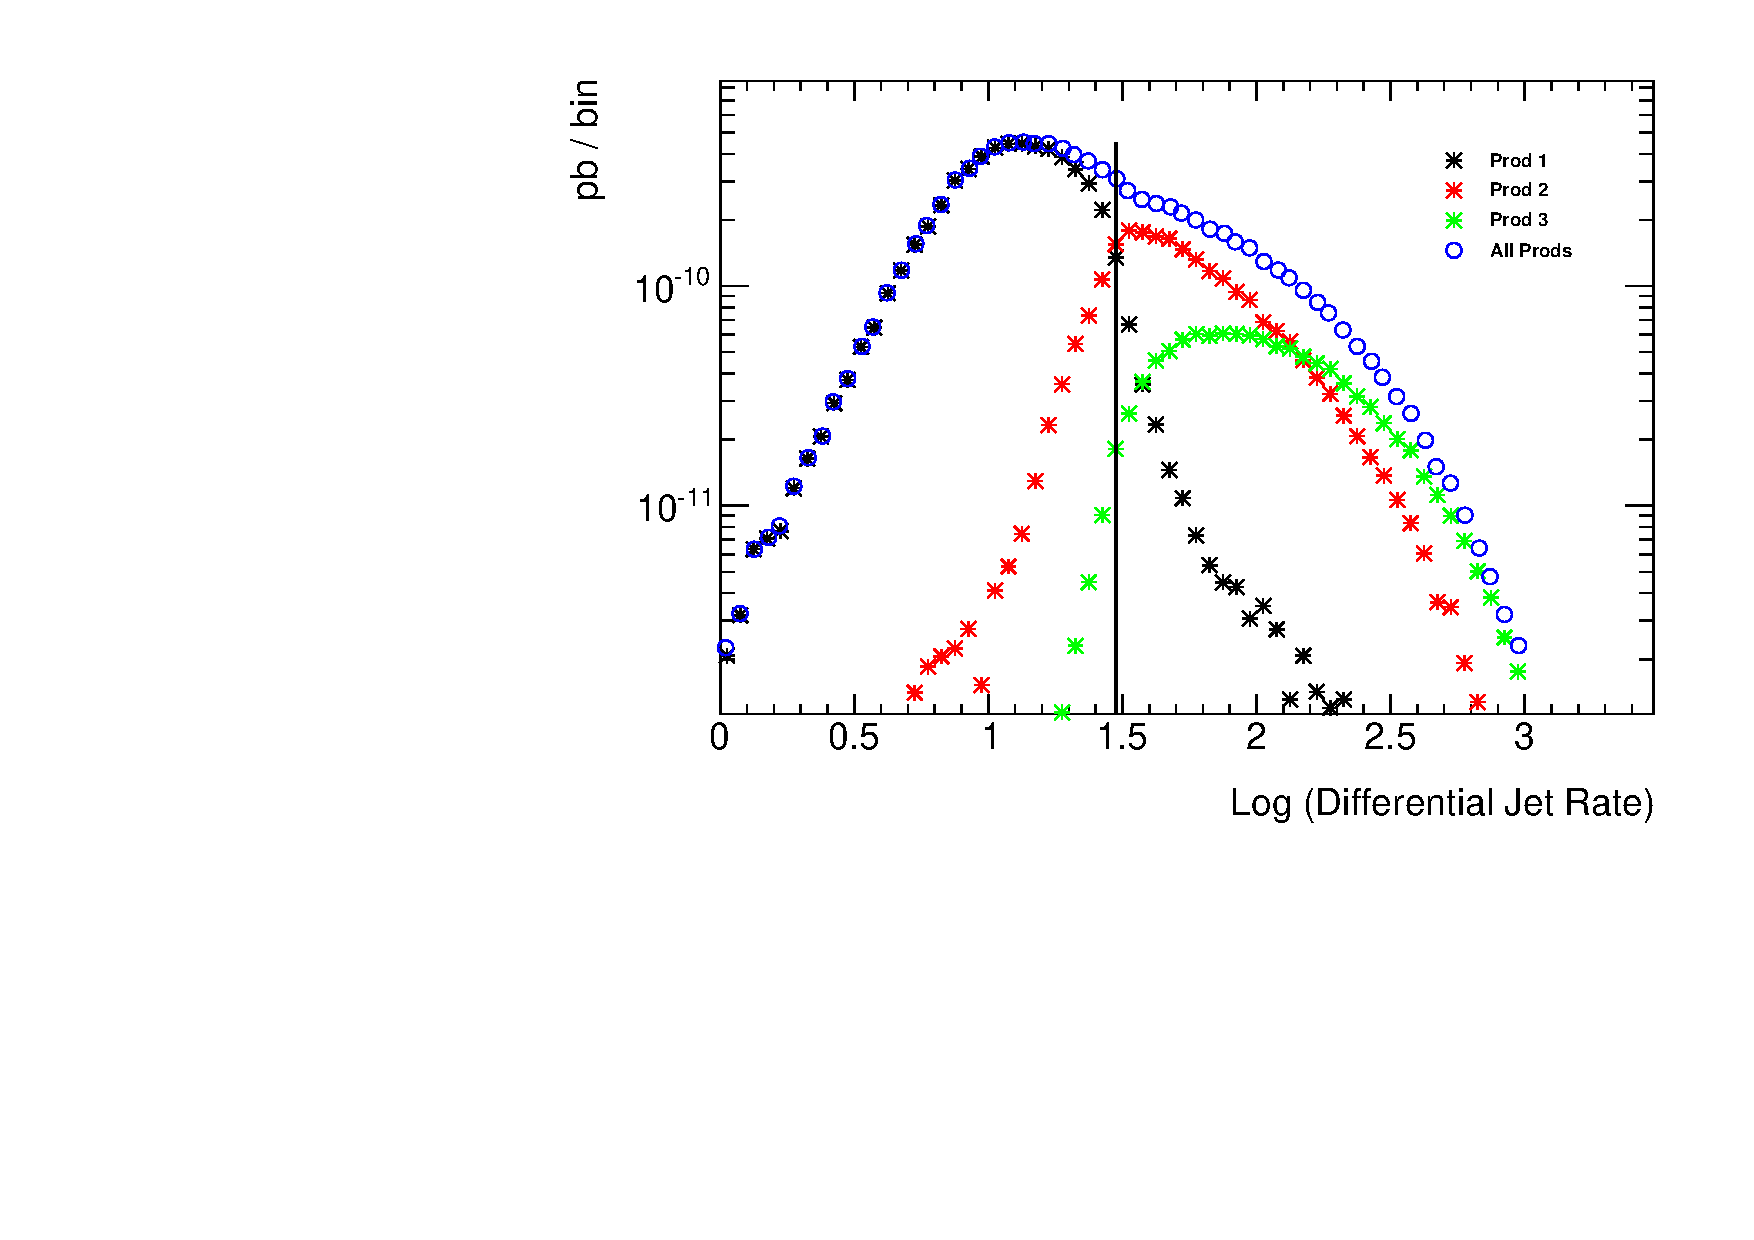
\includegraphics[width=0.48\linewidth]{figures/monojet_appendix/HistoJet1to2_30.pdf}
	}
	\hfill
	\subfloat[$2\rightarrow3$ parton process]{%
		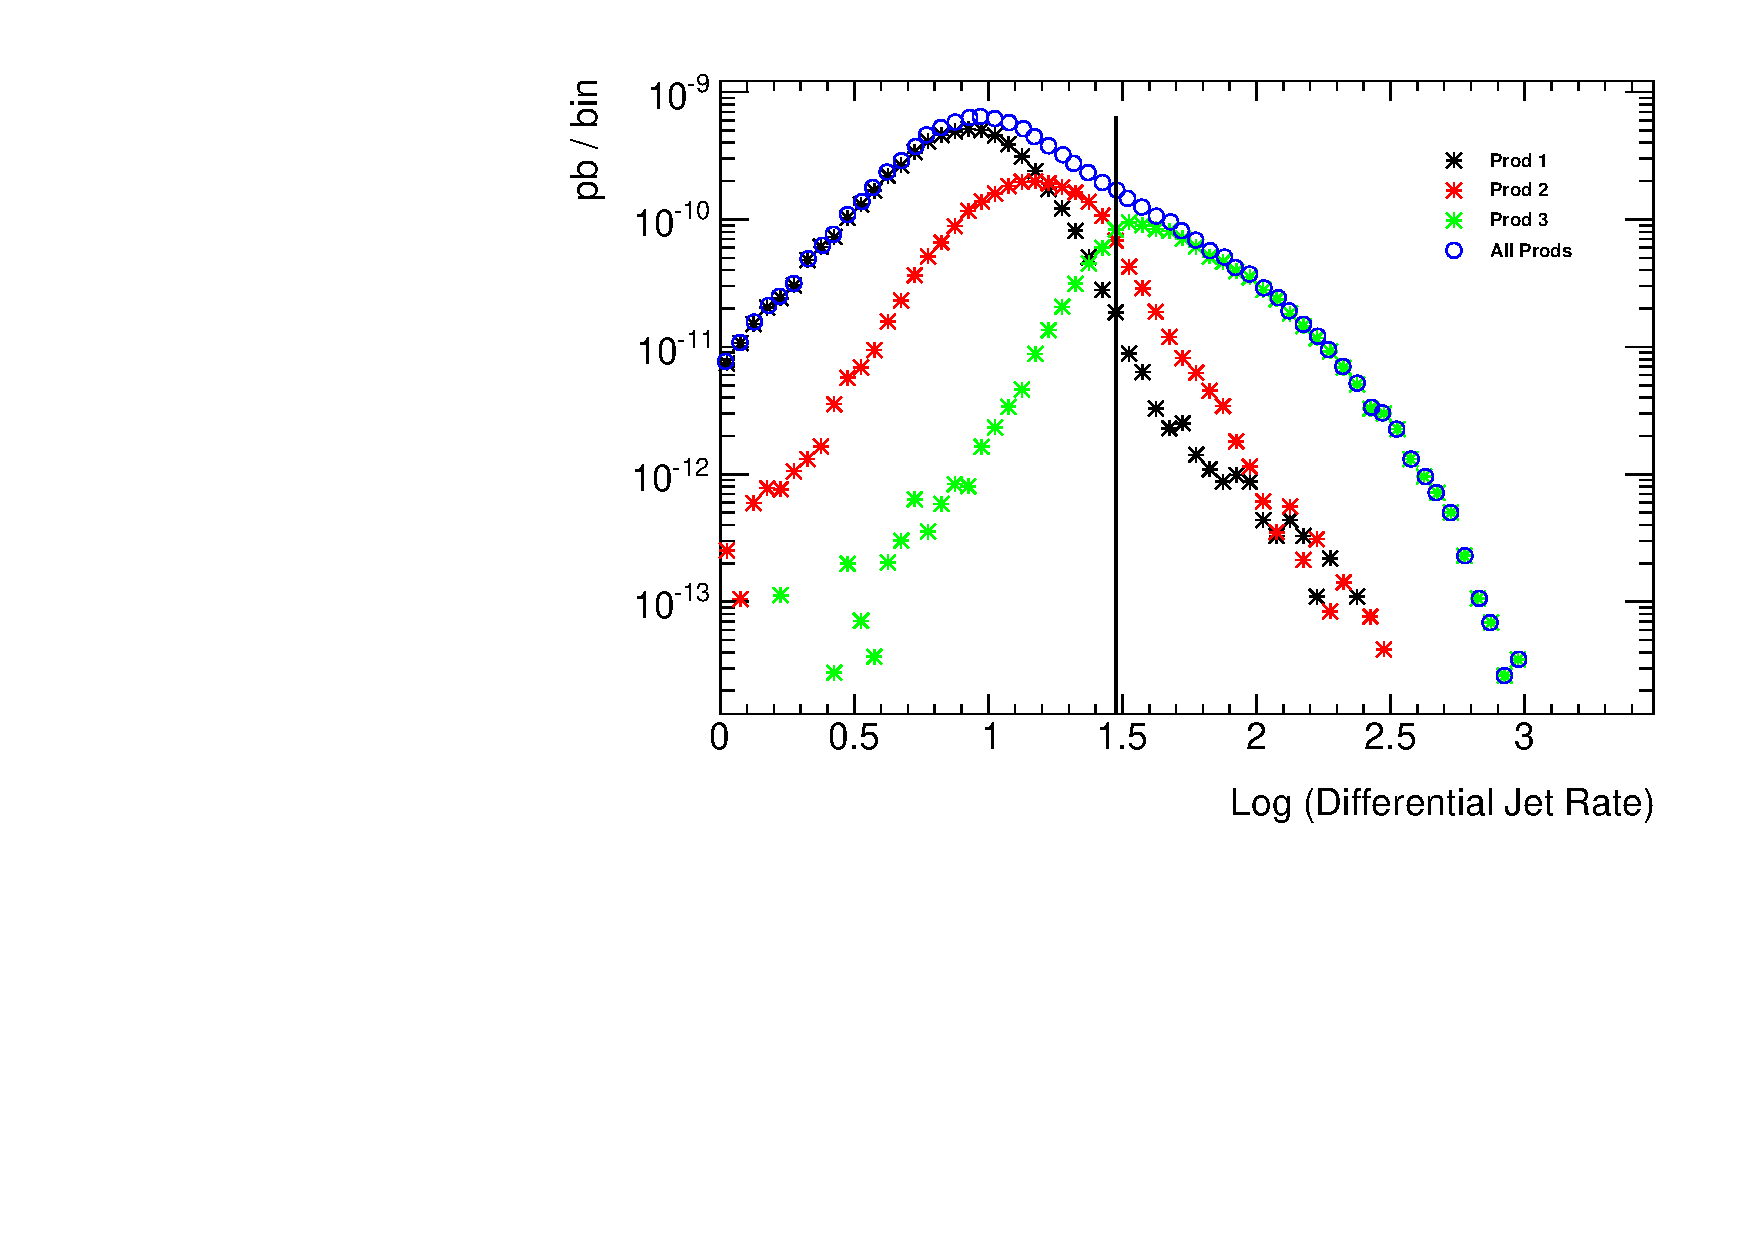
\includegraphics[width=0.48\linewidth]{figures/monojet_appendix/HistoJet2to3_30.pdf}
	}
	\hfill
	\subfloat[$3\rightarrow4$ parton process]{%
		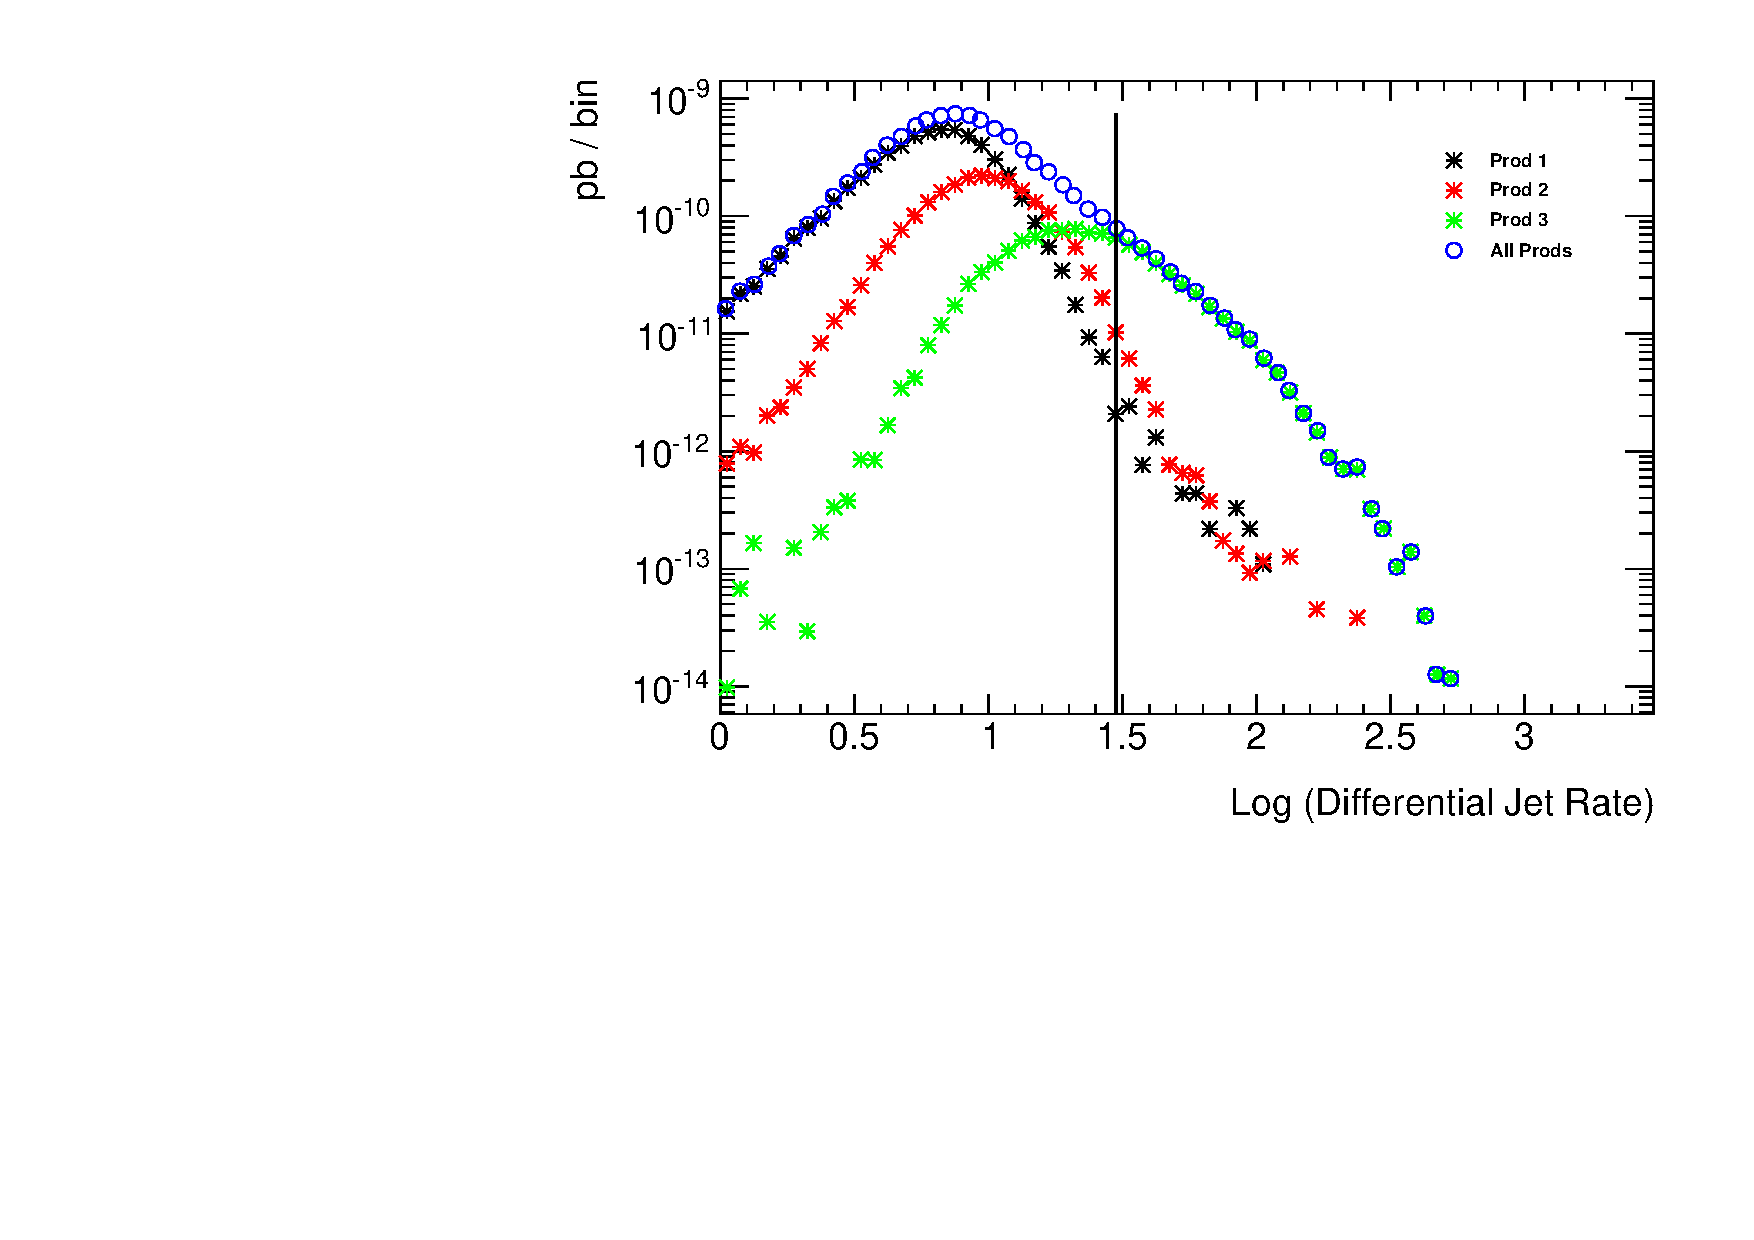
\includegraphics[width=0.48\linewidth]{figures/monojet_appendix/HistoJet3to4_30.pdf}
	}
	\hfill
	\subfloat[$4\rightarrow5$ parton process]{%
		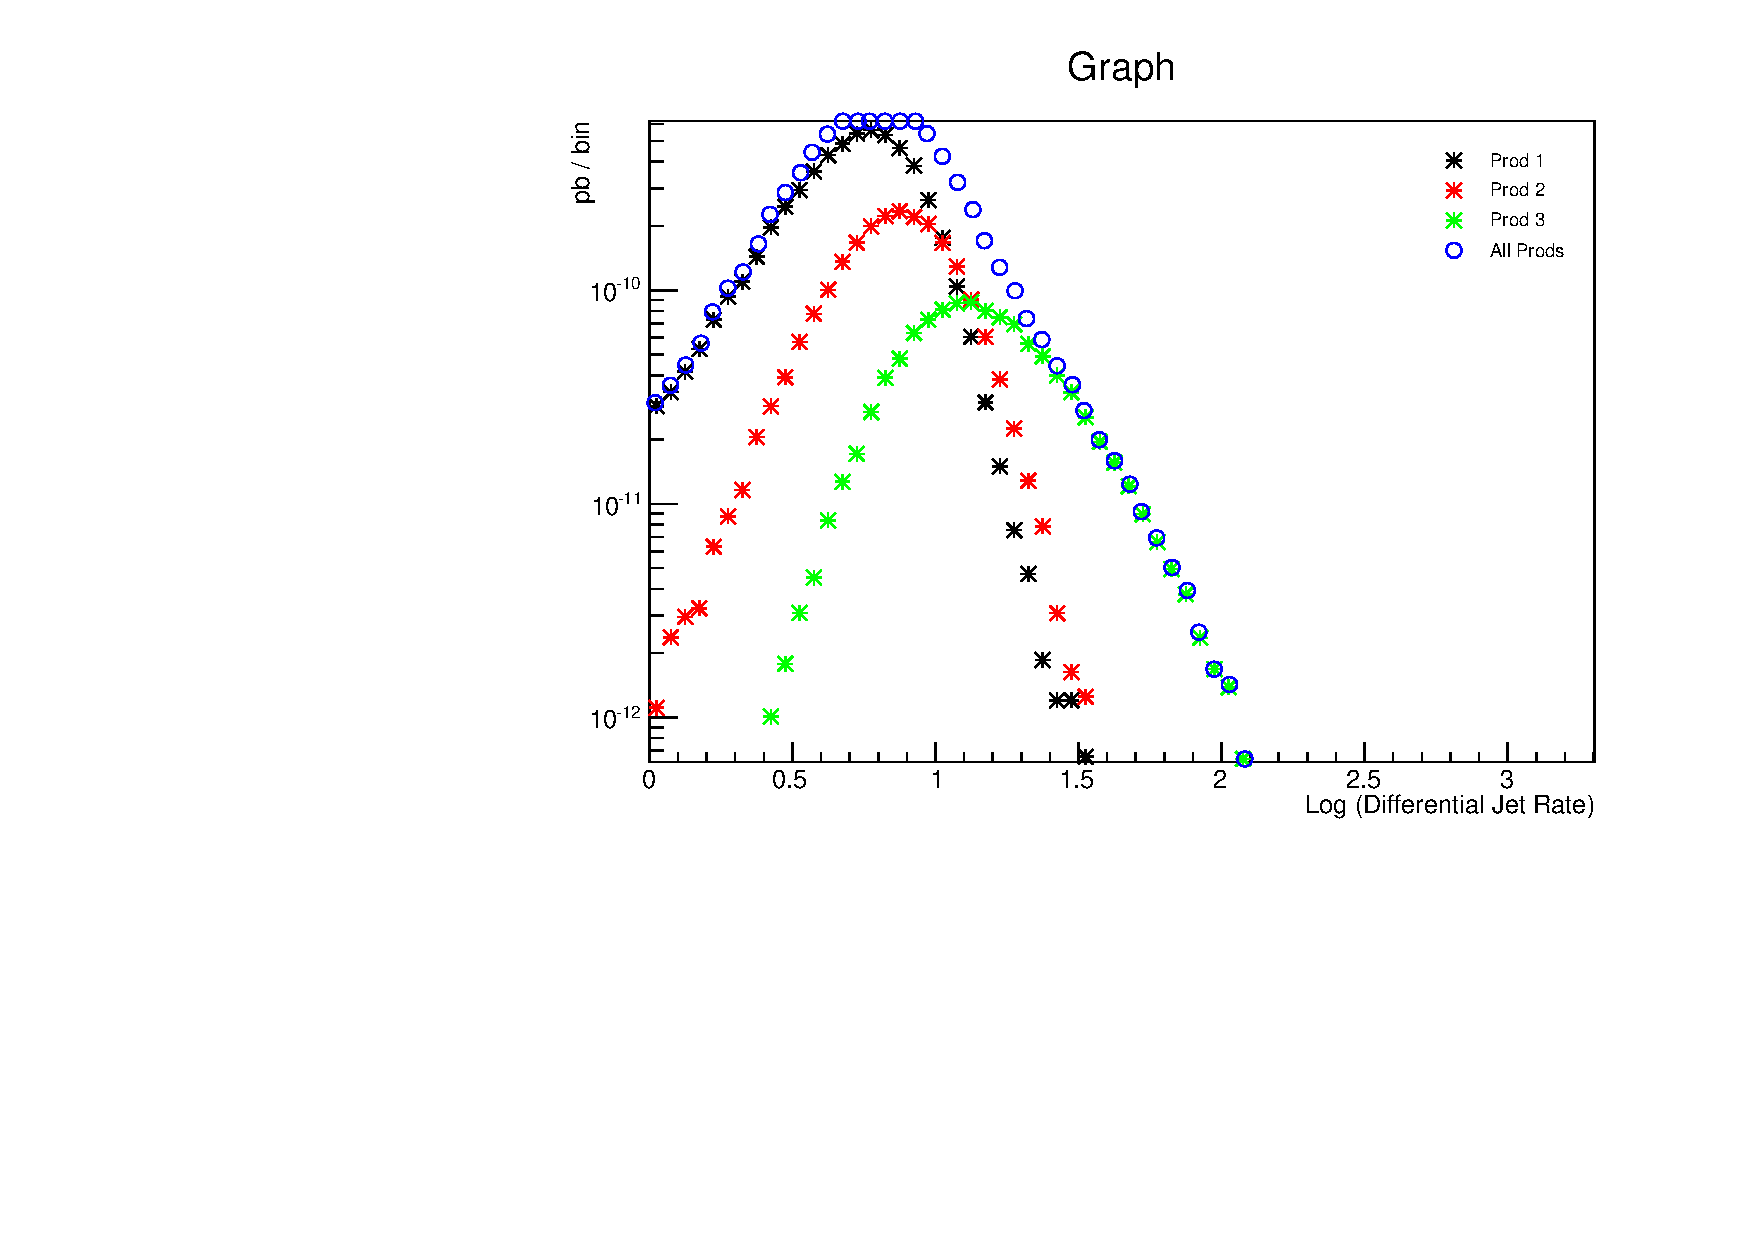
\includegraphics[width=0.48\linewidth]{figures/monojet_appendix/HistoJet4to5_30.pdf}
	}
	\caption{Jet differential rates distributions for EFT D5 sample with CKKW matching scale at 30 GeV. 0-, 1- and 2-parton emission cases are generated separatedly. A vertical line is drawn at the matching scale.}
	\label{fig:CKKW_D5_30}
\end{figure}


\begin{figure}[h!]
	\centering  
	\subfloat[$1\rightarrow2$ parton process]{%
		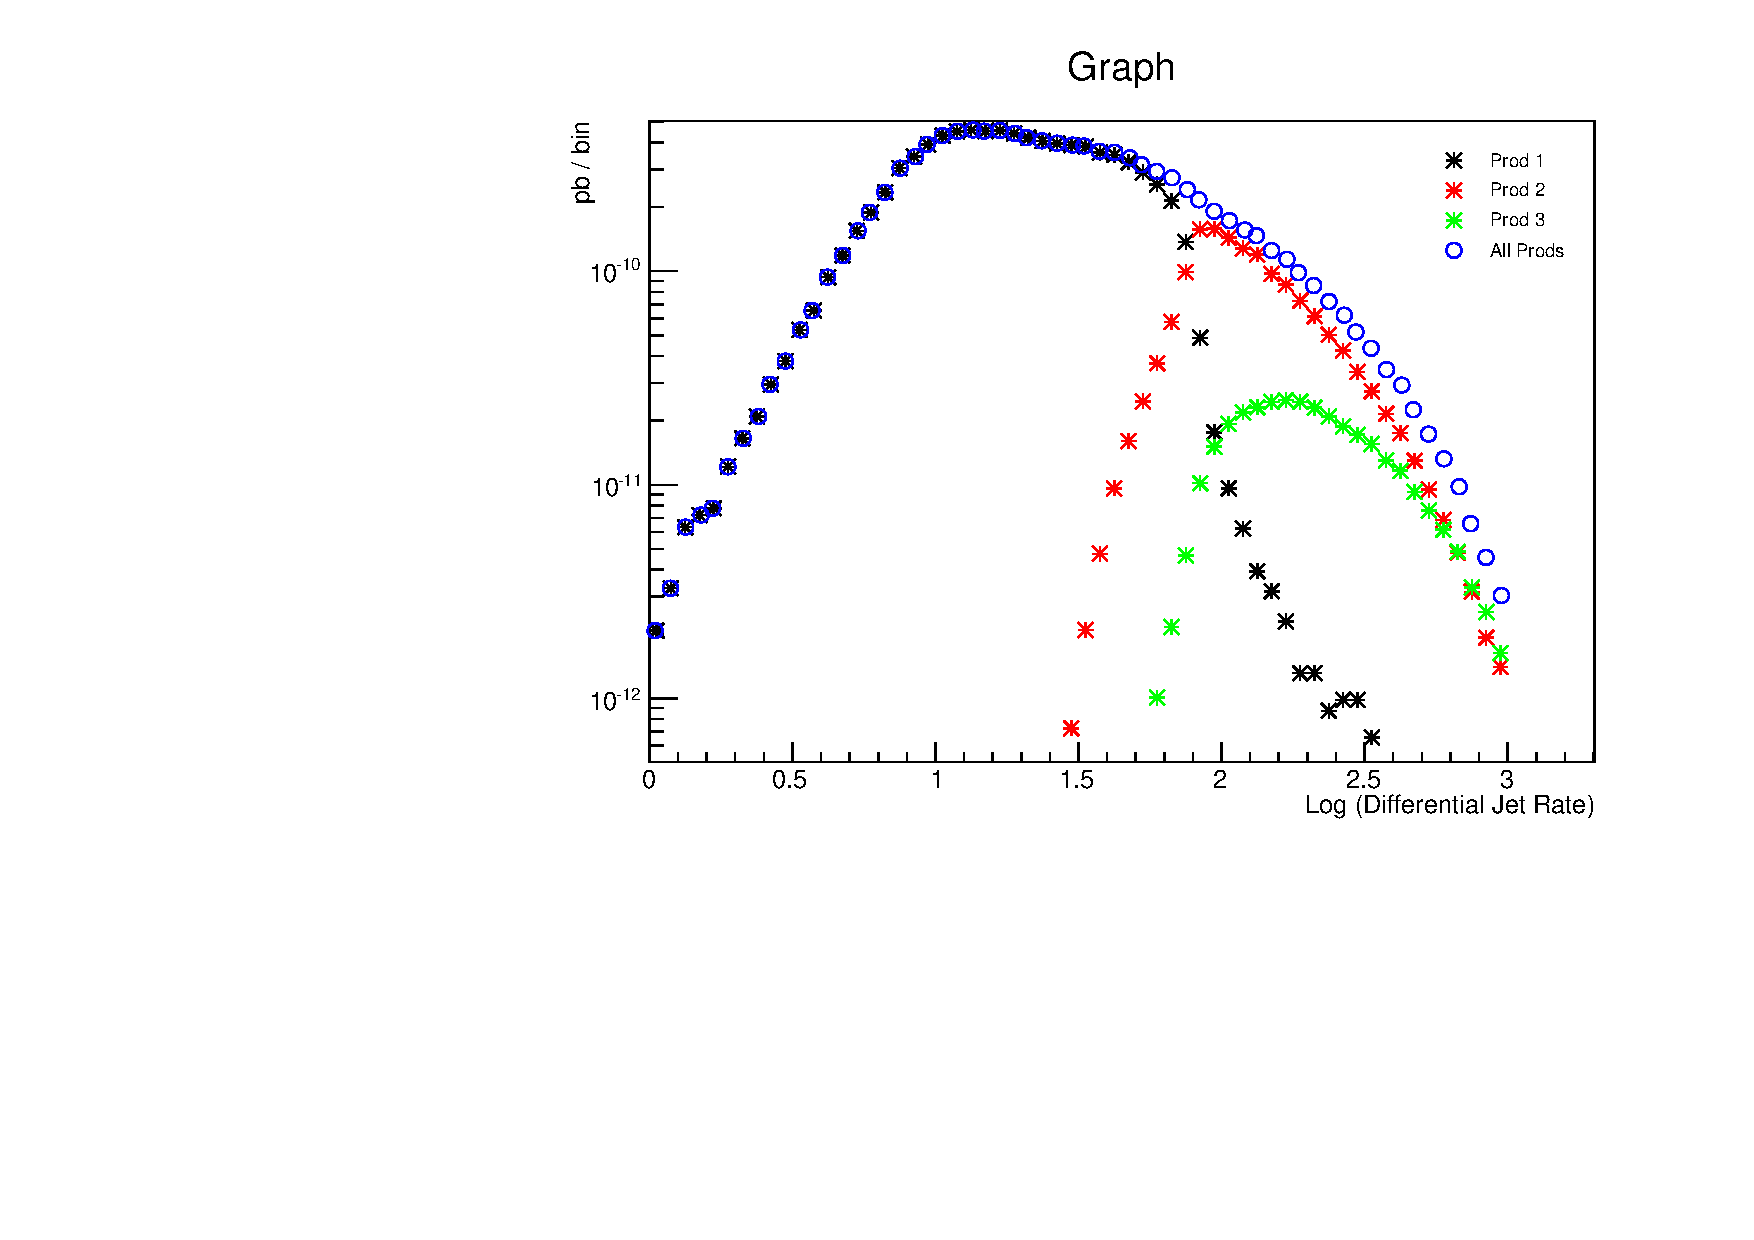
\includegraphics[width=0.48\linewidth]{figures/monojet_appendix/HistoJet1to2_80.pdf}
	}
	\hfill
	\subfloat[$2\rightarrow3$ parton process]{%
		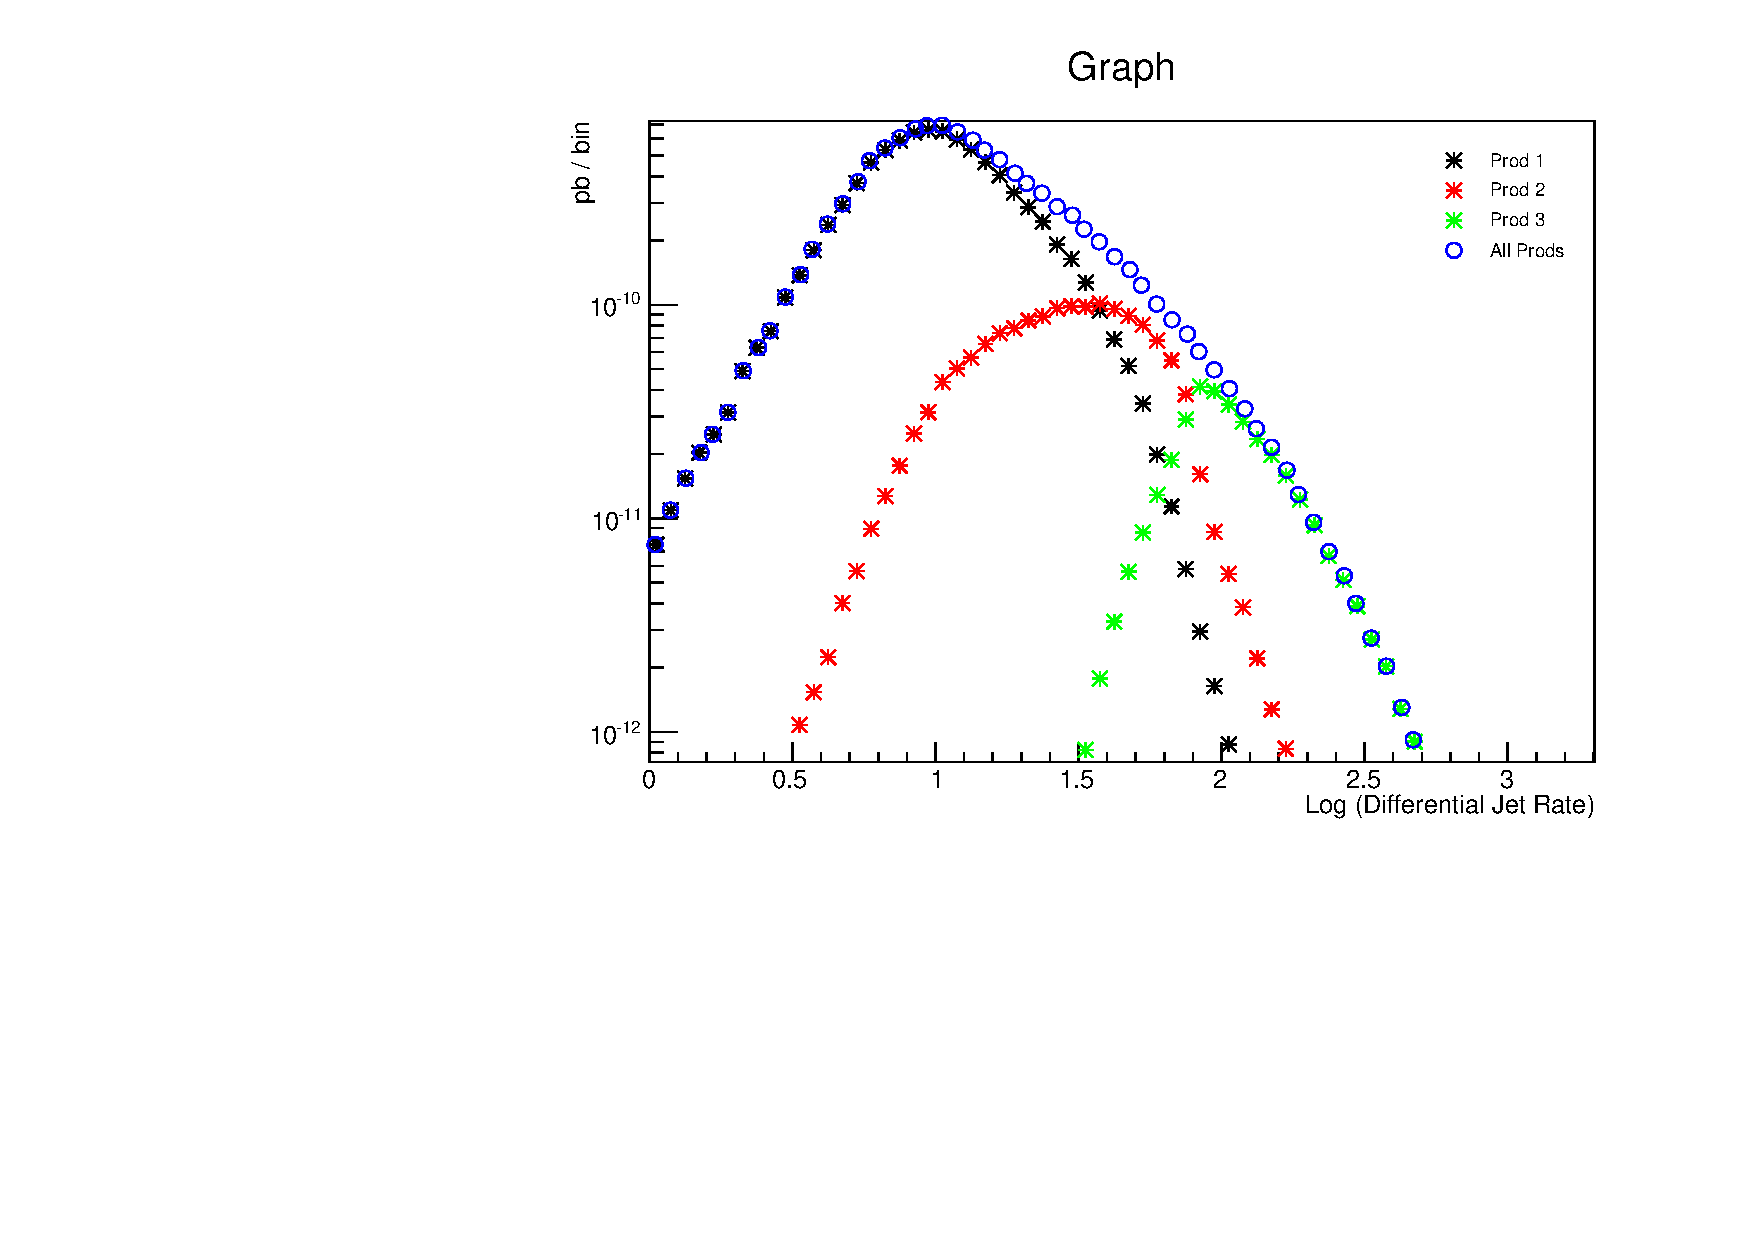
\includegraphics[width=0.48\linewidth]{figures/monojet_appendix/HistoJet2to3_80.pdf}
	}
	\hfill
	\subfloat[$3\rightarrow4$ parton process]{%
    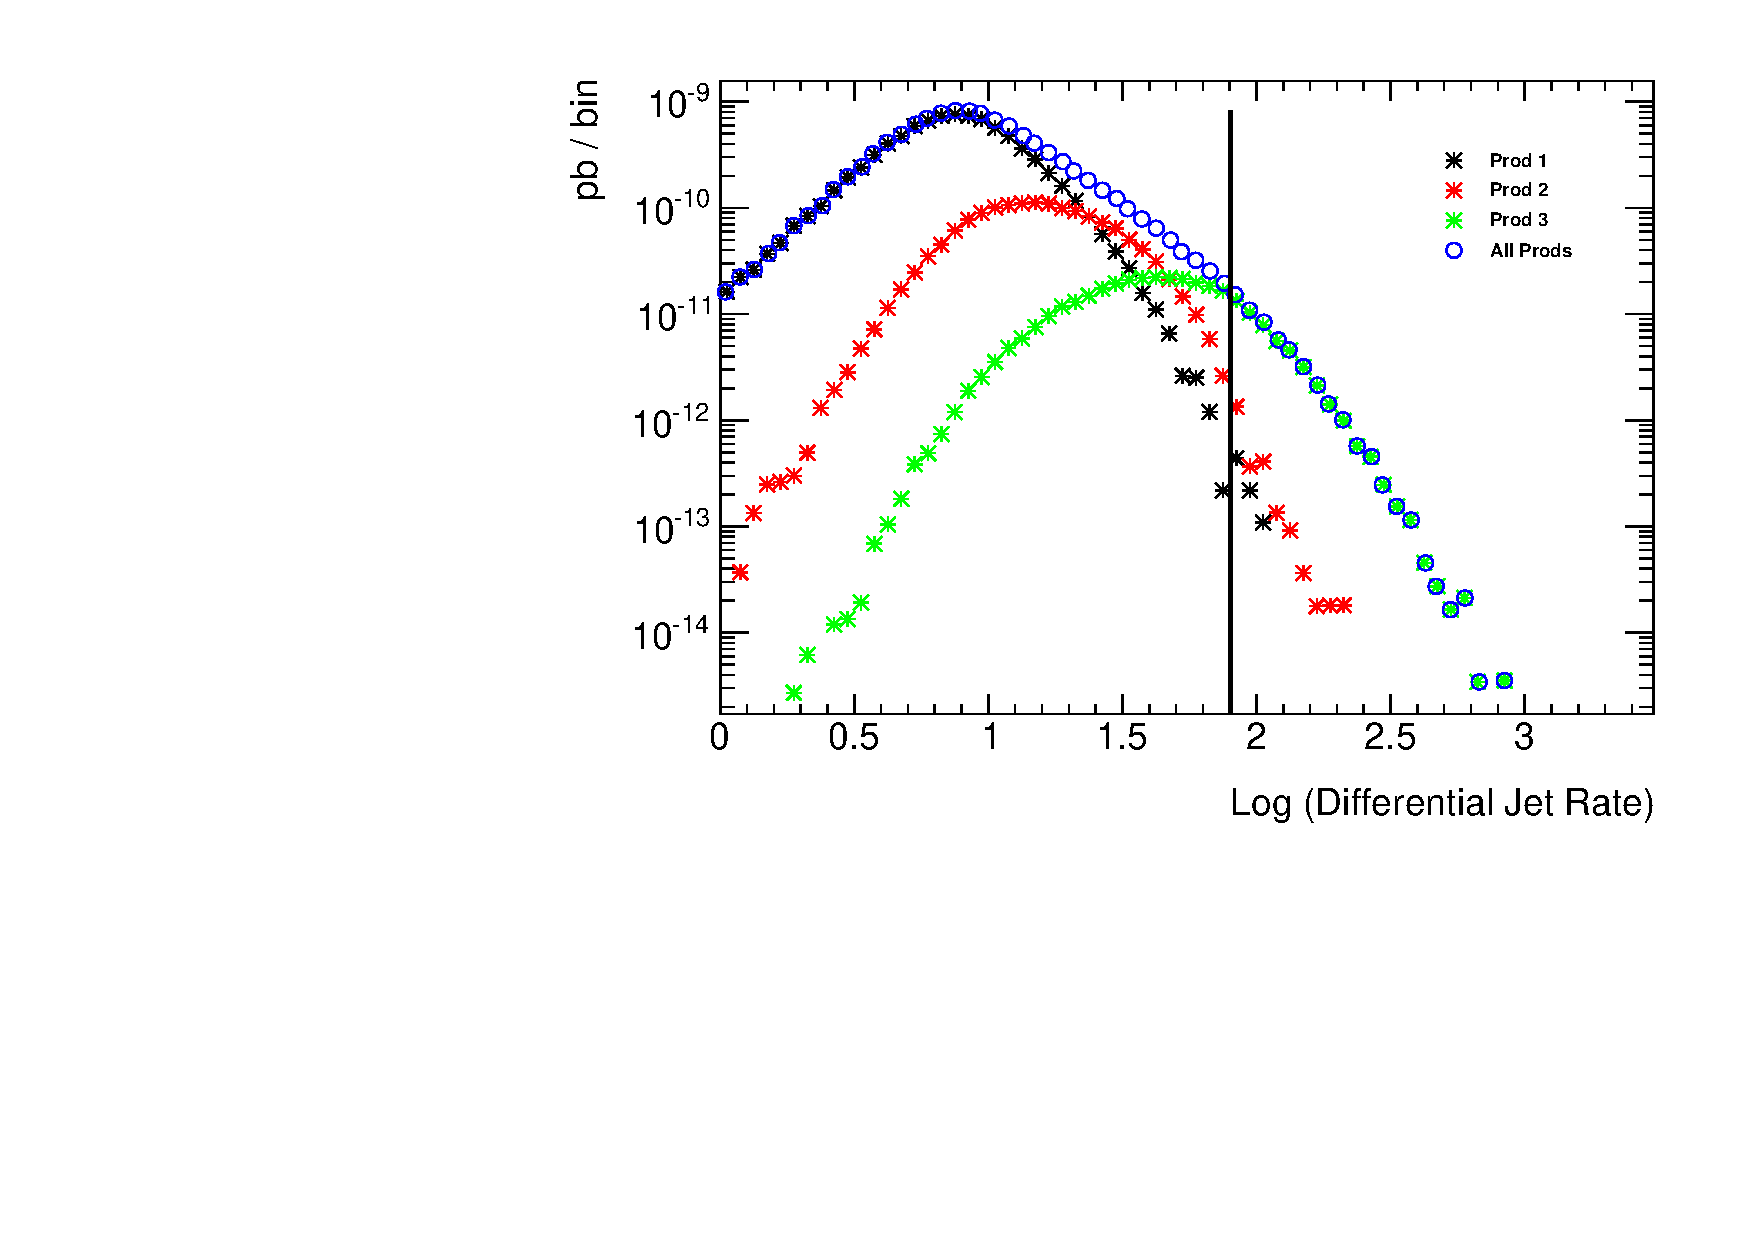
\includegraphics[width=0.48\linewidth]{figures/monojet_appendix/HistoJet3to4_80.pdf}
	}
	\hfill
	\subfloat[$4\rightarrow5$ parton process]{%
    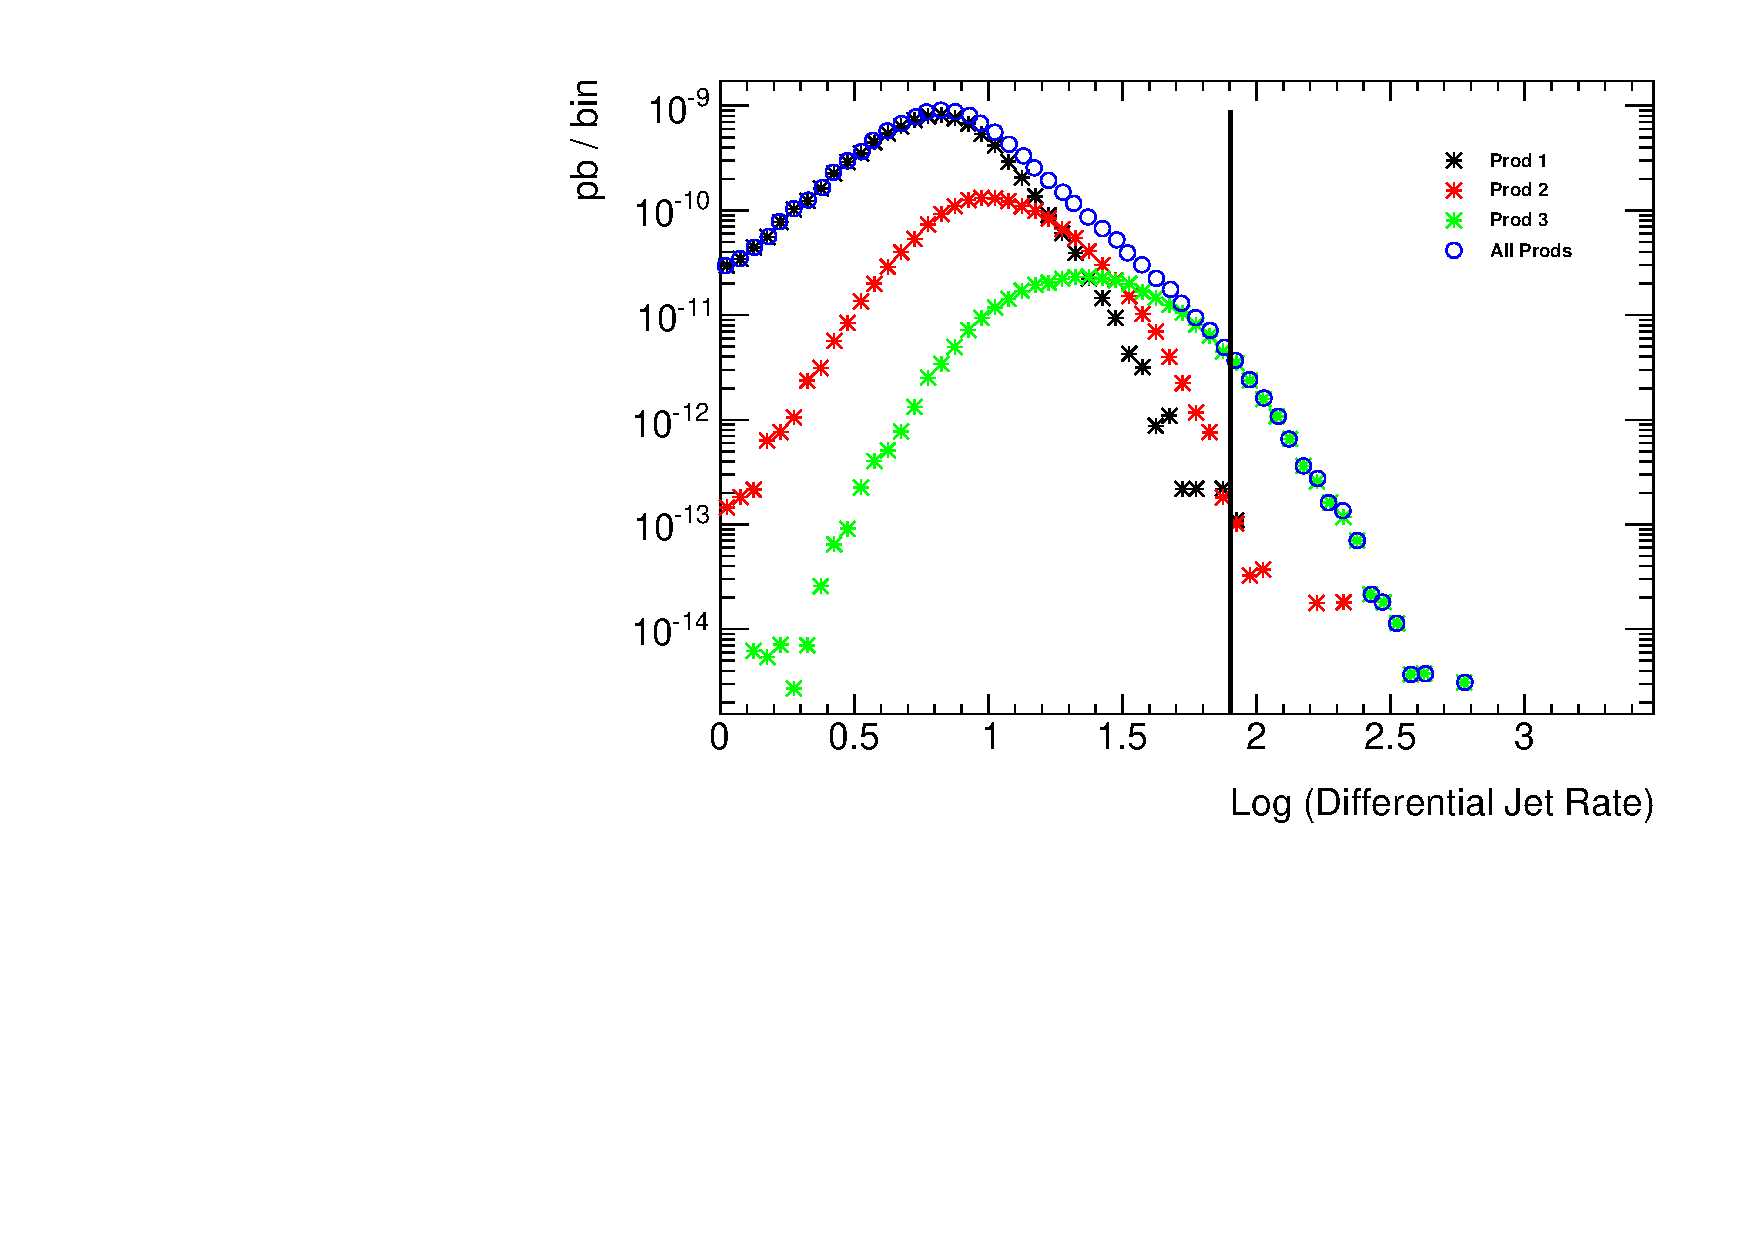
\includegraphics[width=0.48\linewidth]{figures/monojet_appendix/HistoJet4to5_80.pdf}
	}
  \caption{Jet differential rates distributions for EFT D5 sample with CKKW matching scale at 80 GeV. 0-, 1- and 2-parton emission cases are generated separatedly. A vertical line is drawn at the matching scale.}
  \label{fig:CKKW_D5_80}
\end{figure}

To compare the effect in a finer step, the matching scales at 30, 50, 70, 80 and 90 GeV are plotted in Fig\ref{fig:CKKW_D5_zoom}. Globally good agreement is seen among different matching scales, with some difference observed around the matching scale. A closer look in this range shows that the 80 and 90 GeV matching scales produce very close distributions, so it is safe to use 80 GeV as the baseline matching scale.

\begin{figure}[h!]
	\centering  
	\subfloat[$1\rightarrow2$ parton process]{%
		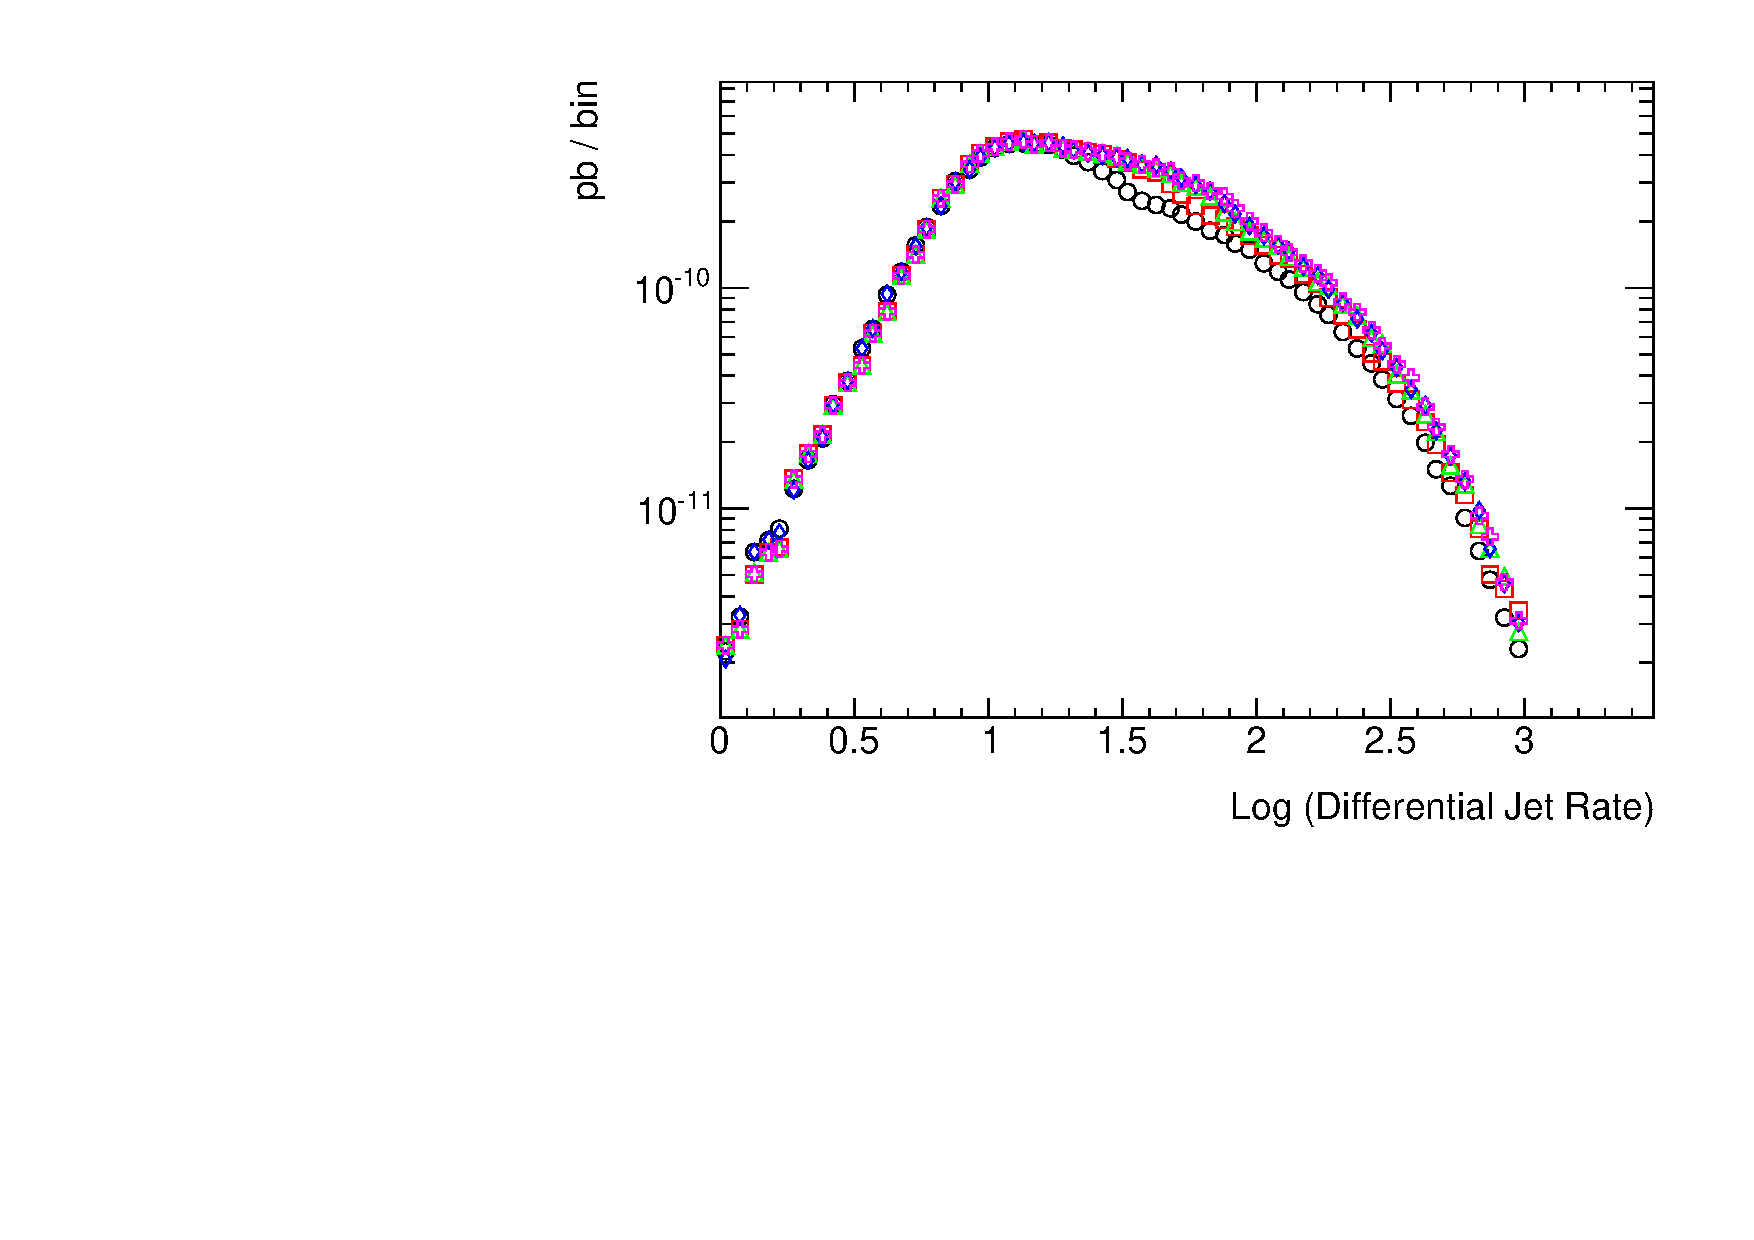
\includegraphics[width=0.48\linewidth]{figures/monojet_appendix/compare_plot_1.pdf}
		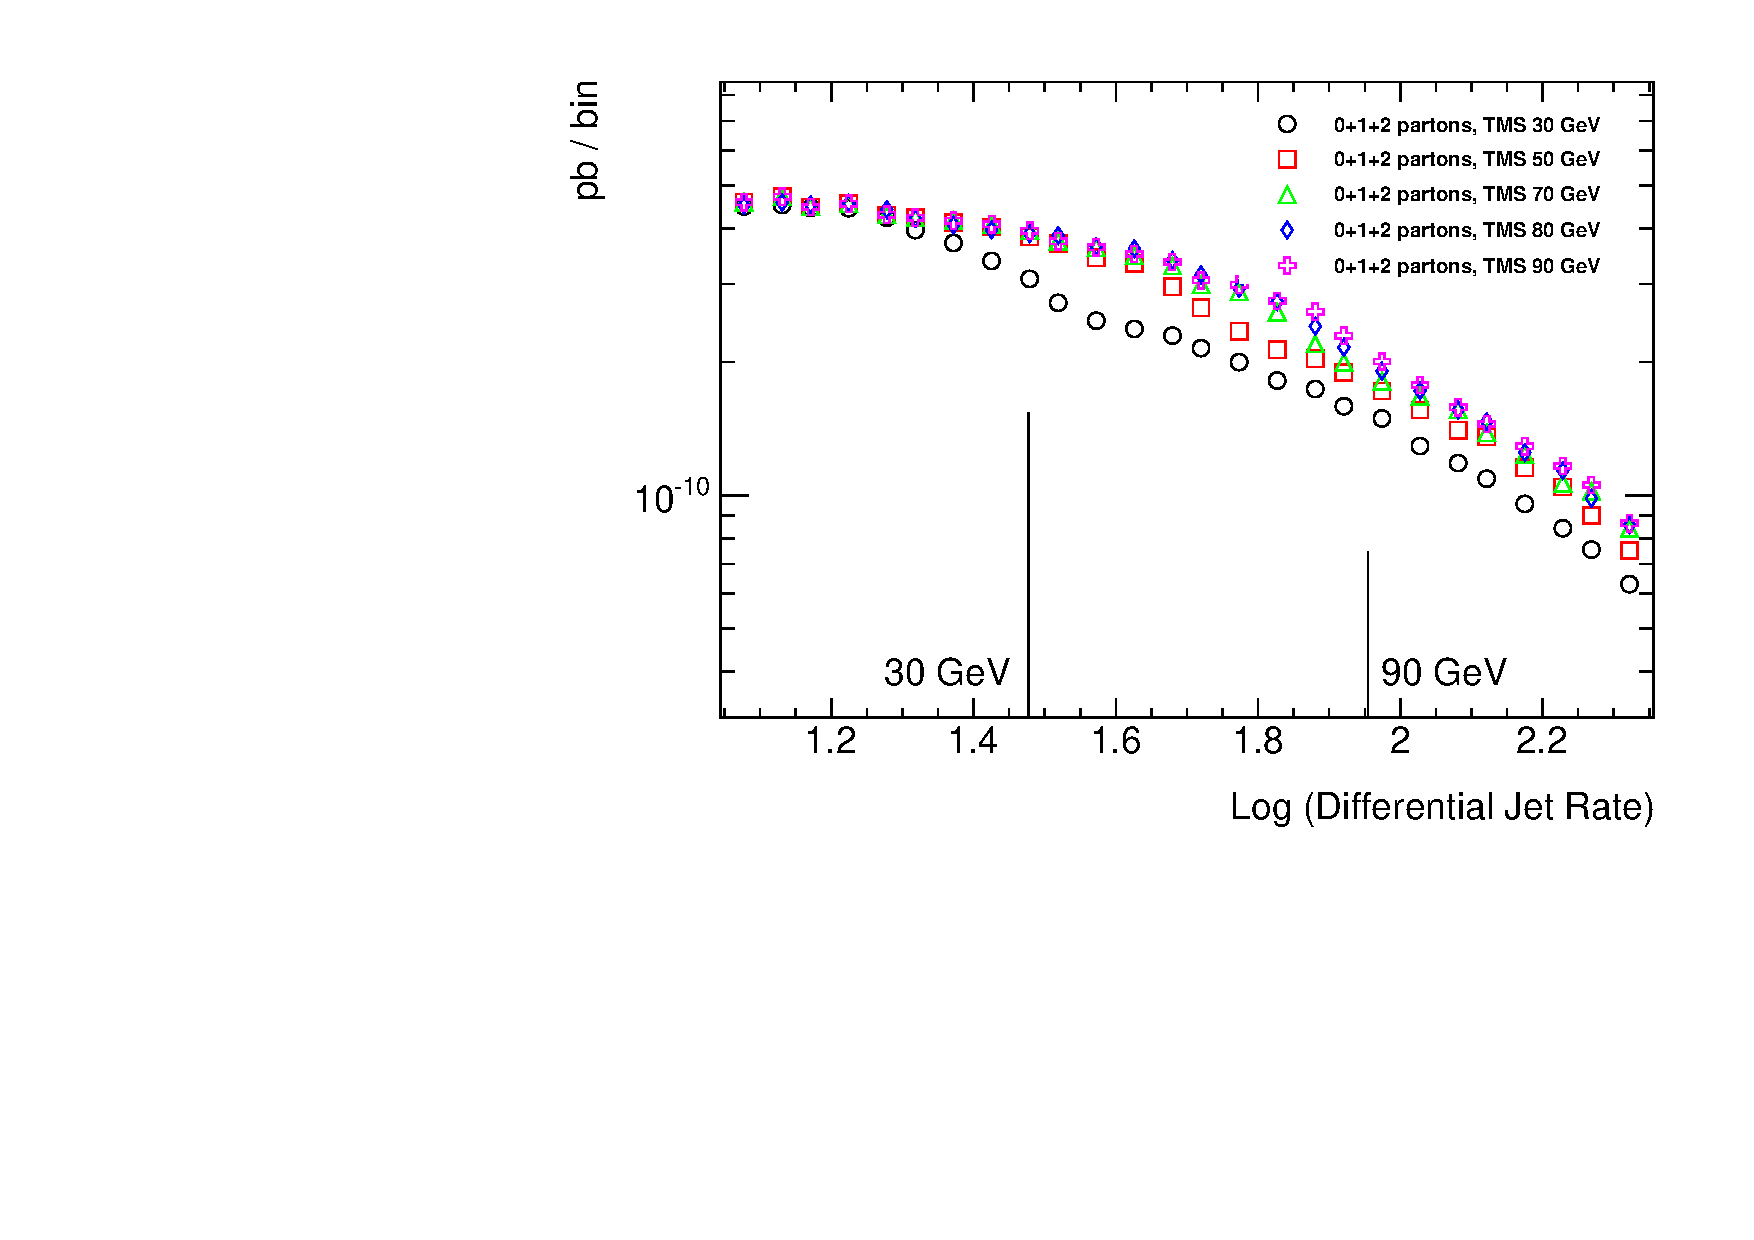
\includegraphics[width=0.48\linewidth]{figures/monojet_appendix/window_plot_1.pdf}
	}
	\hfill
	\subfloat[$2\rightarrow3$ parton process]{%
		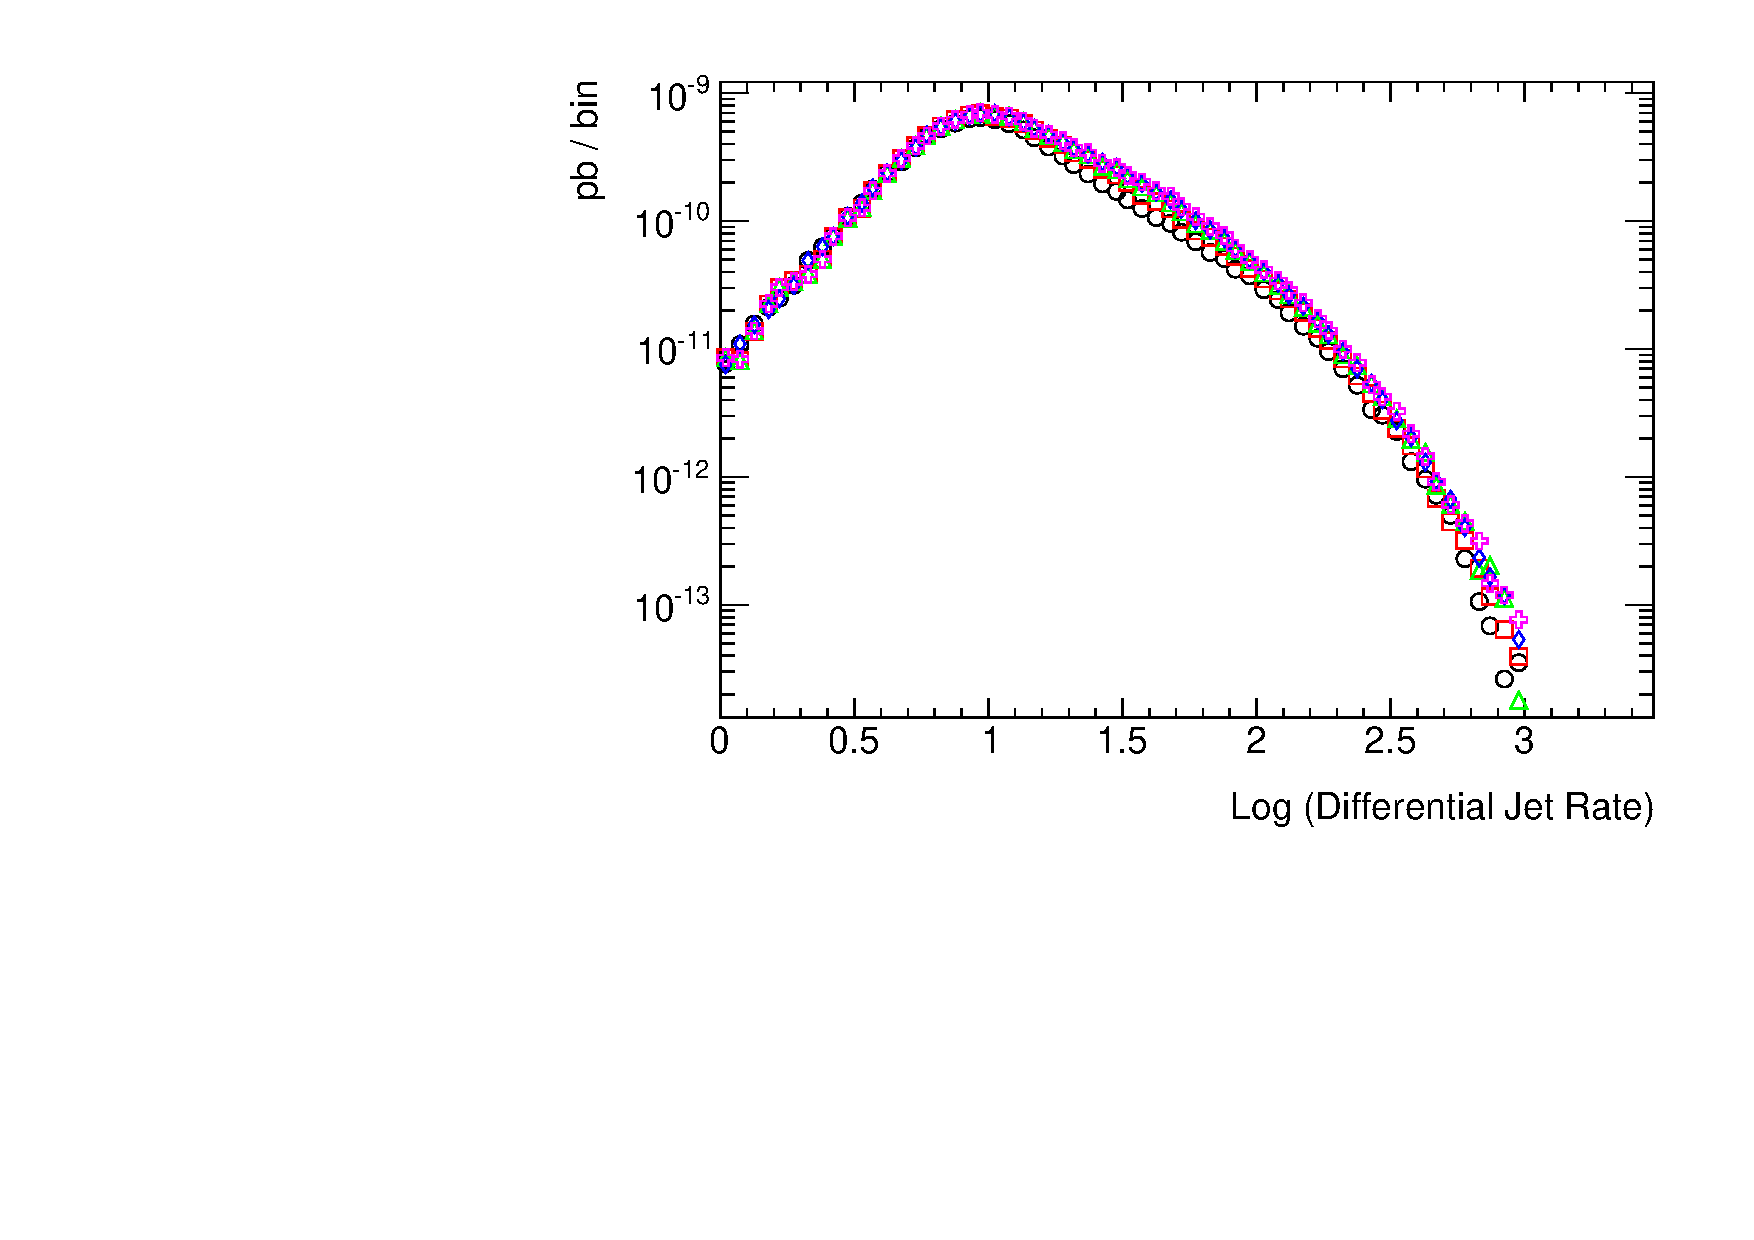
\includegraphics[width=0.48\linewidth]{figures/monojet_appendix/compare_plot_2.pdf}
		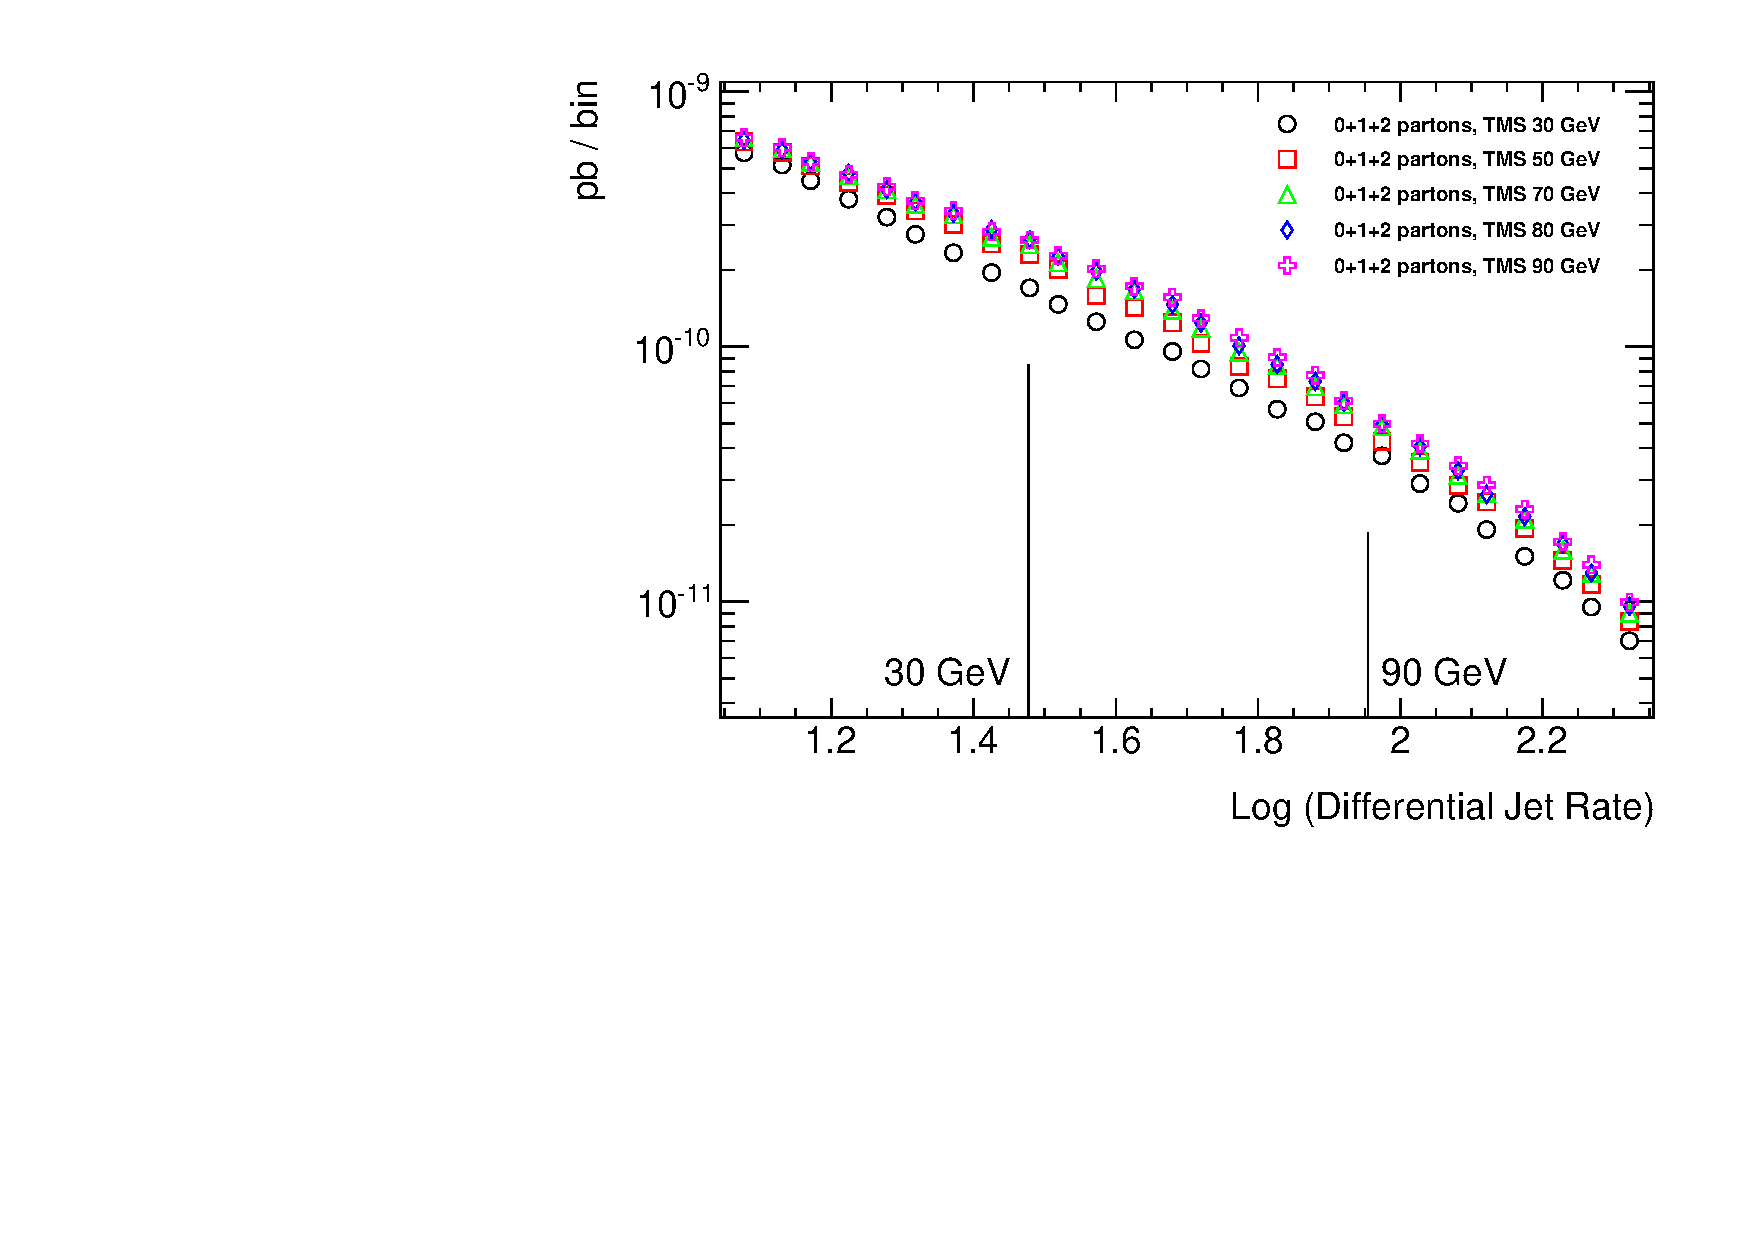
\includegraphics[width=0.48\linewidth]{figures/monojet_appendix/window_plot_2.pdf}
	}
	\hfill
	\subfloat[$3\rightarrow4$ parton process]{%
		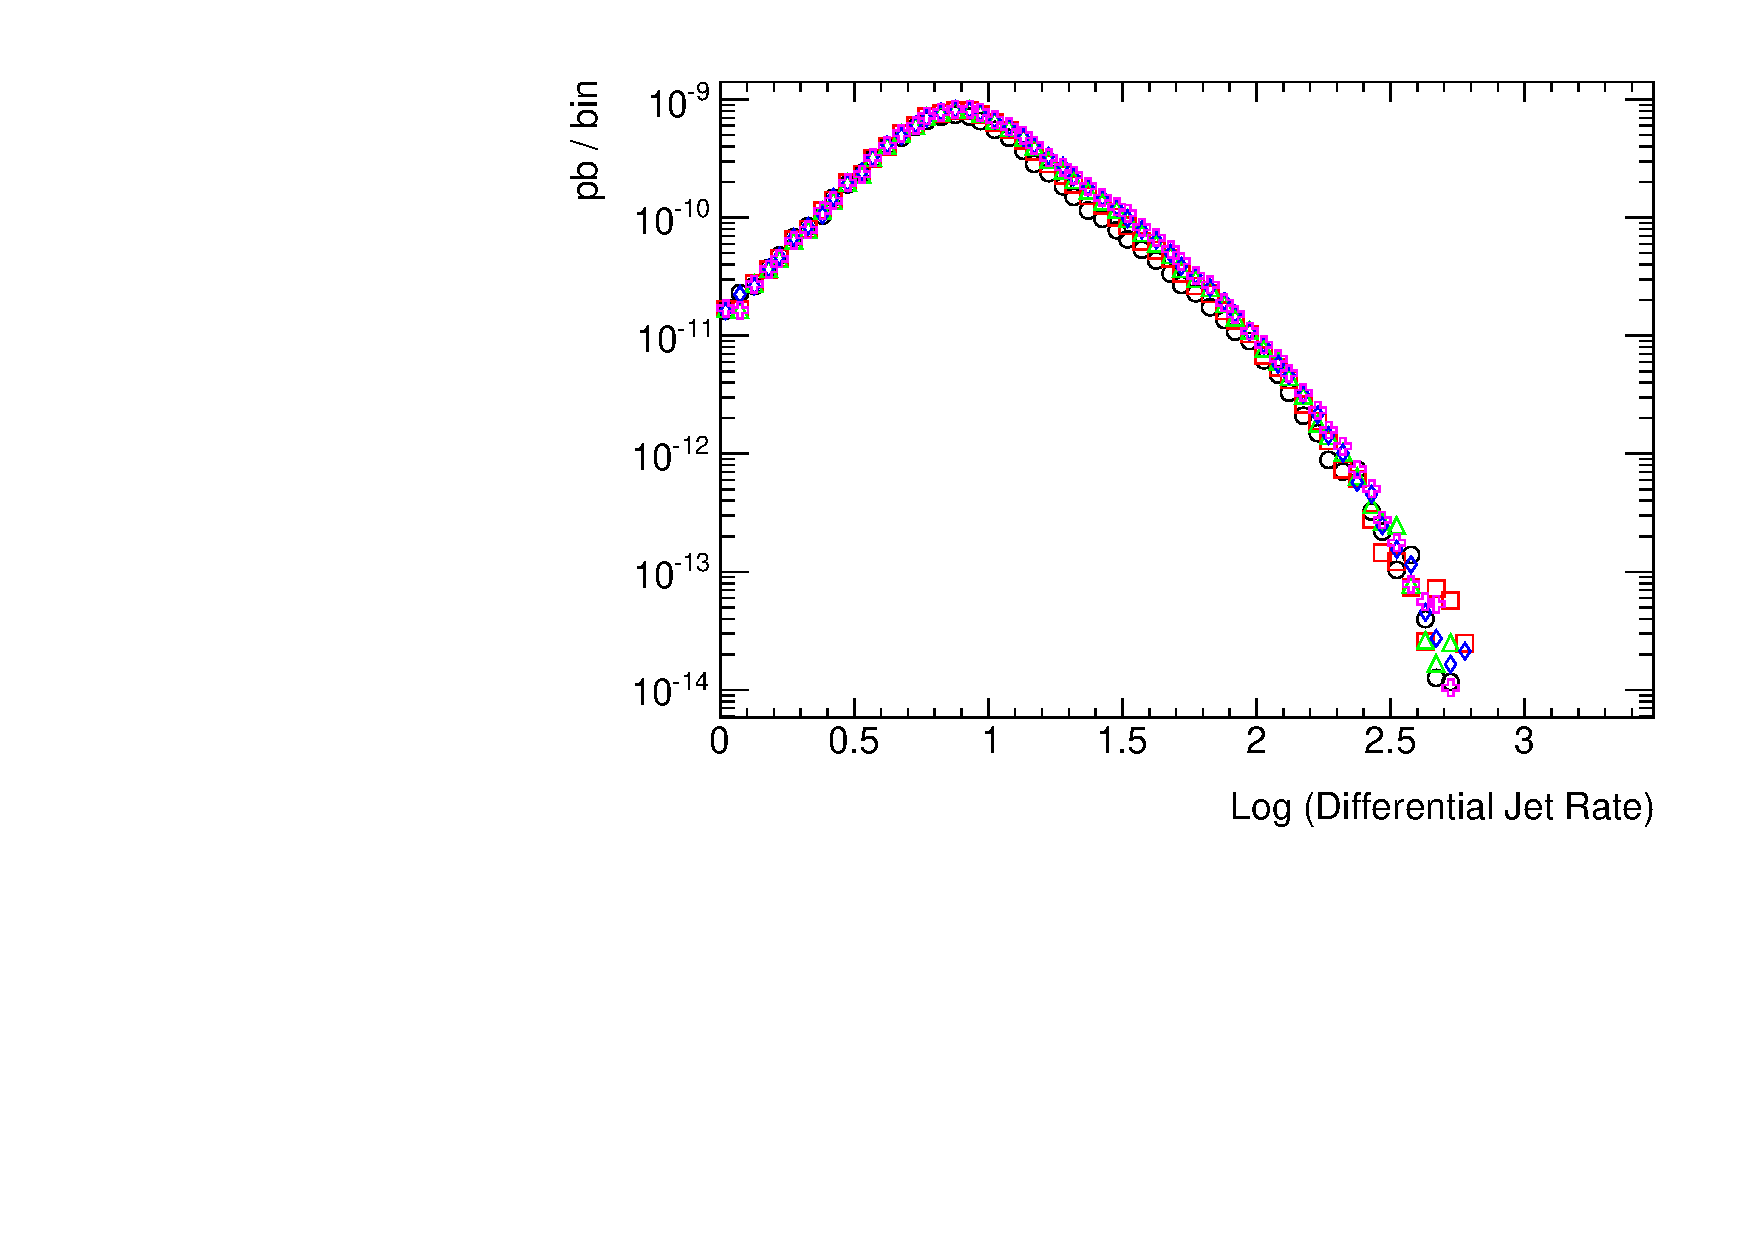
\includegraphics[width=0.48\linewidth]{figures/monojet_appendix/compare_plot_3.pdf}
		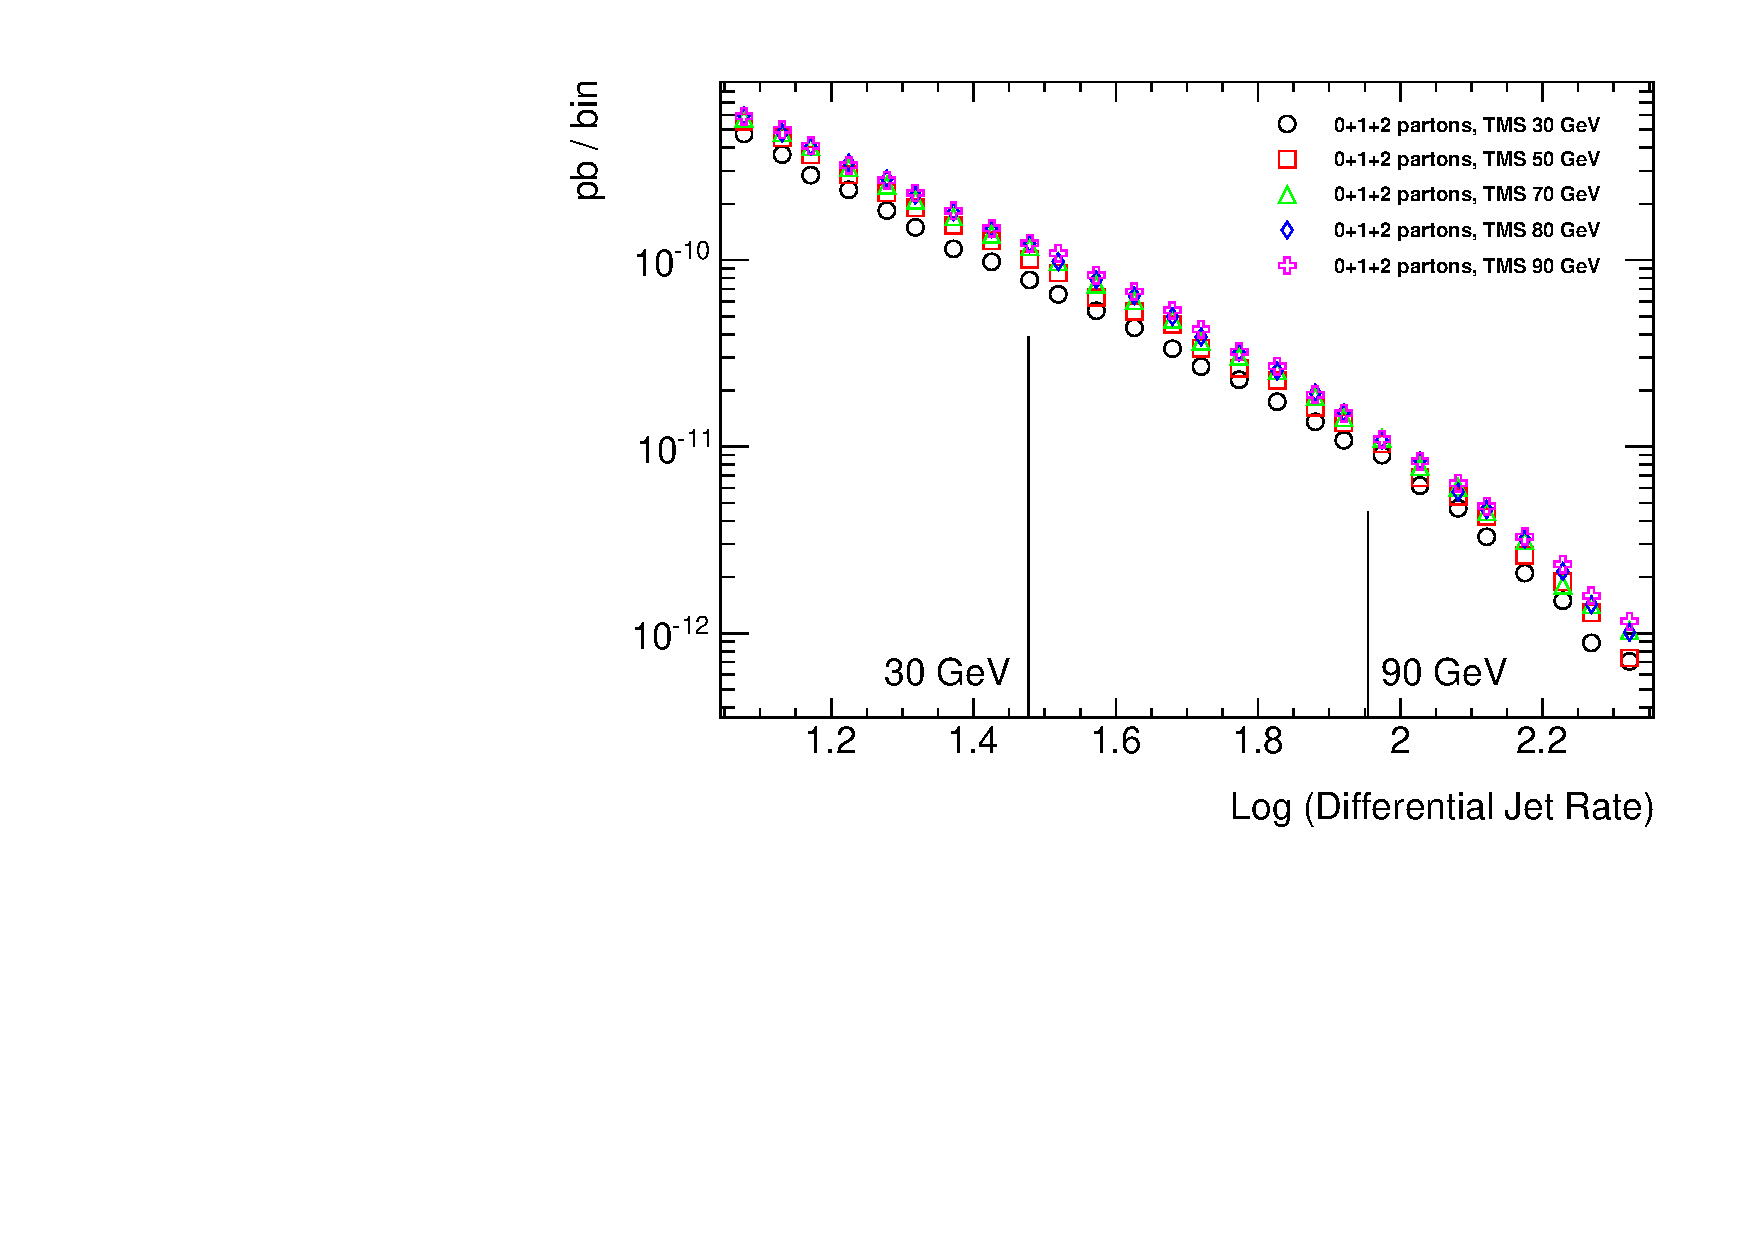
\includegraphics[width=0.48\linewidth]{figures/monojet_appendix/window_plot_3.pdf}
	}
	\hfill
	\subfloat[$4\rightarrow5$ parton process]{%
		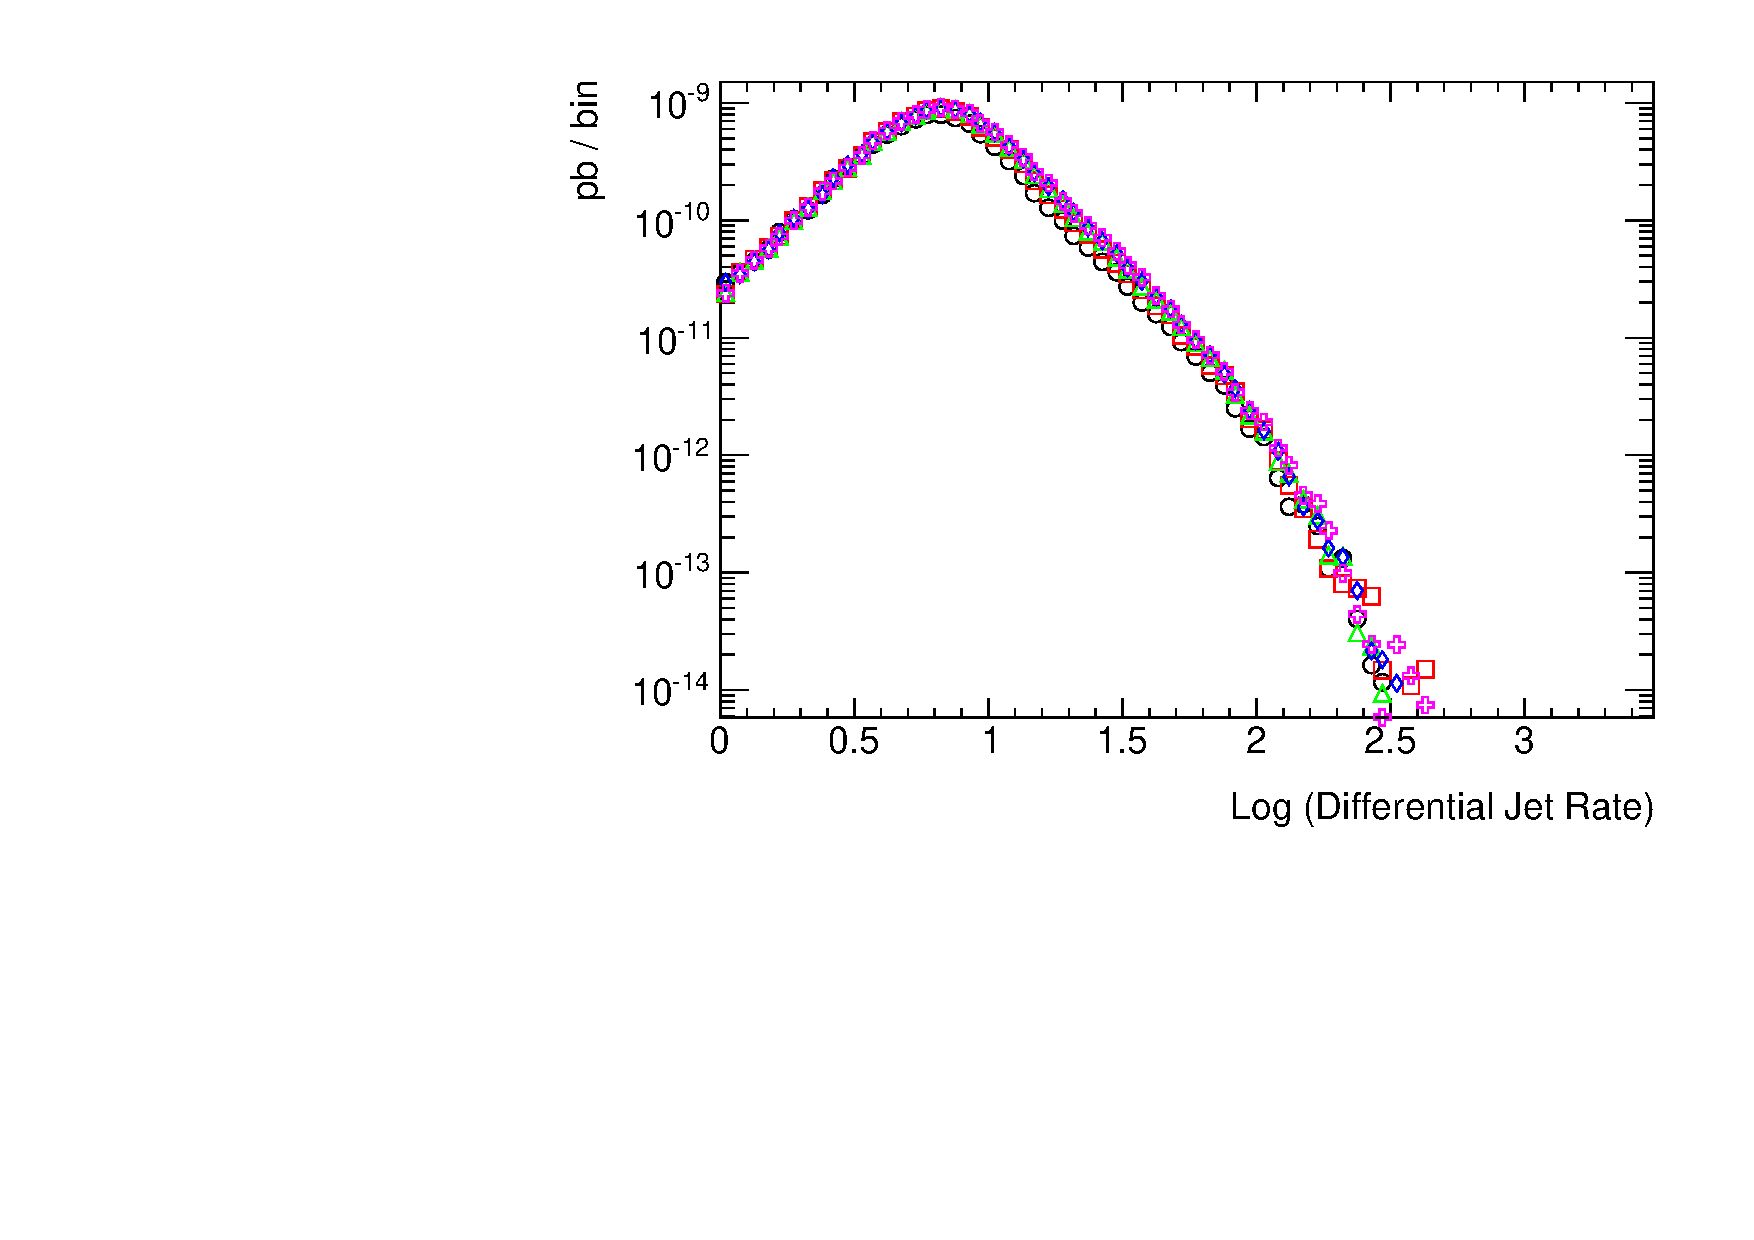
\includegraphics[width=0.48\linewidth]{figures/monojet_appendix/compare_plot_4.pdf}
		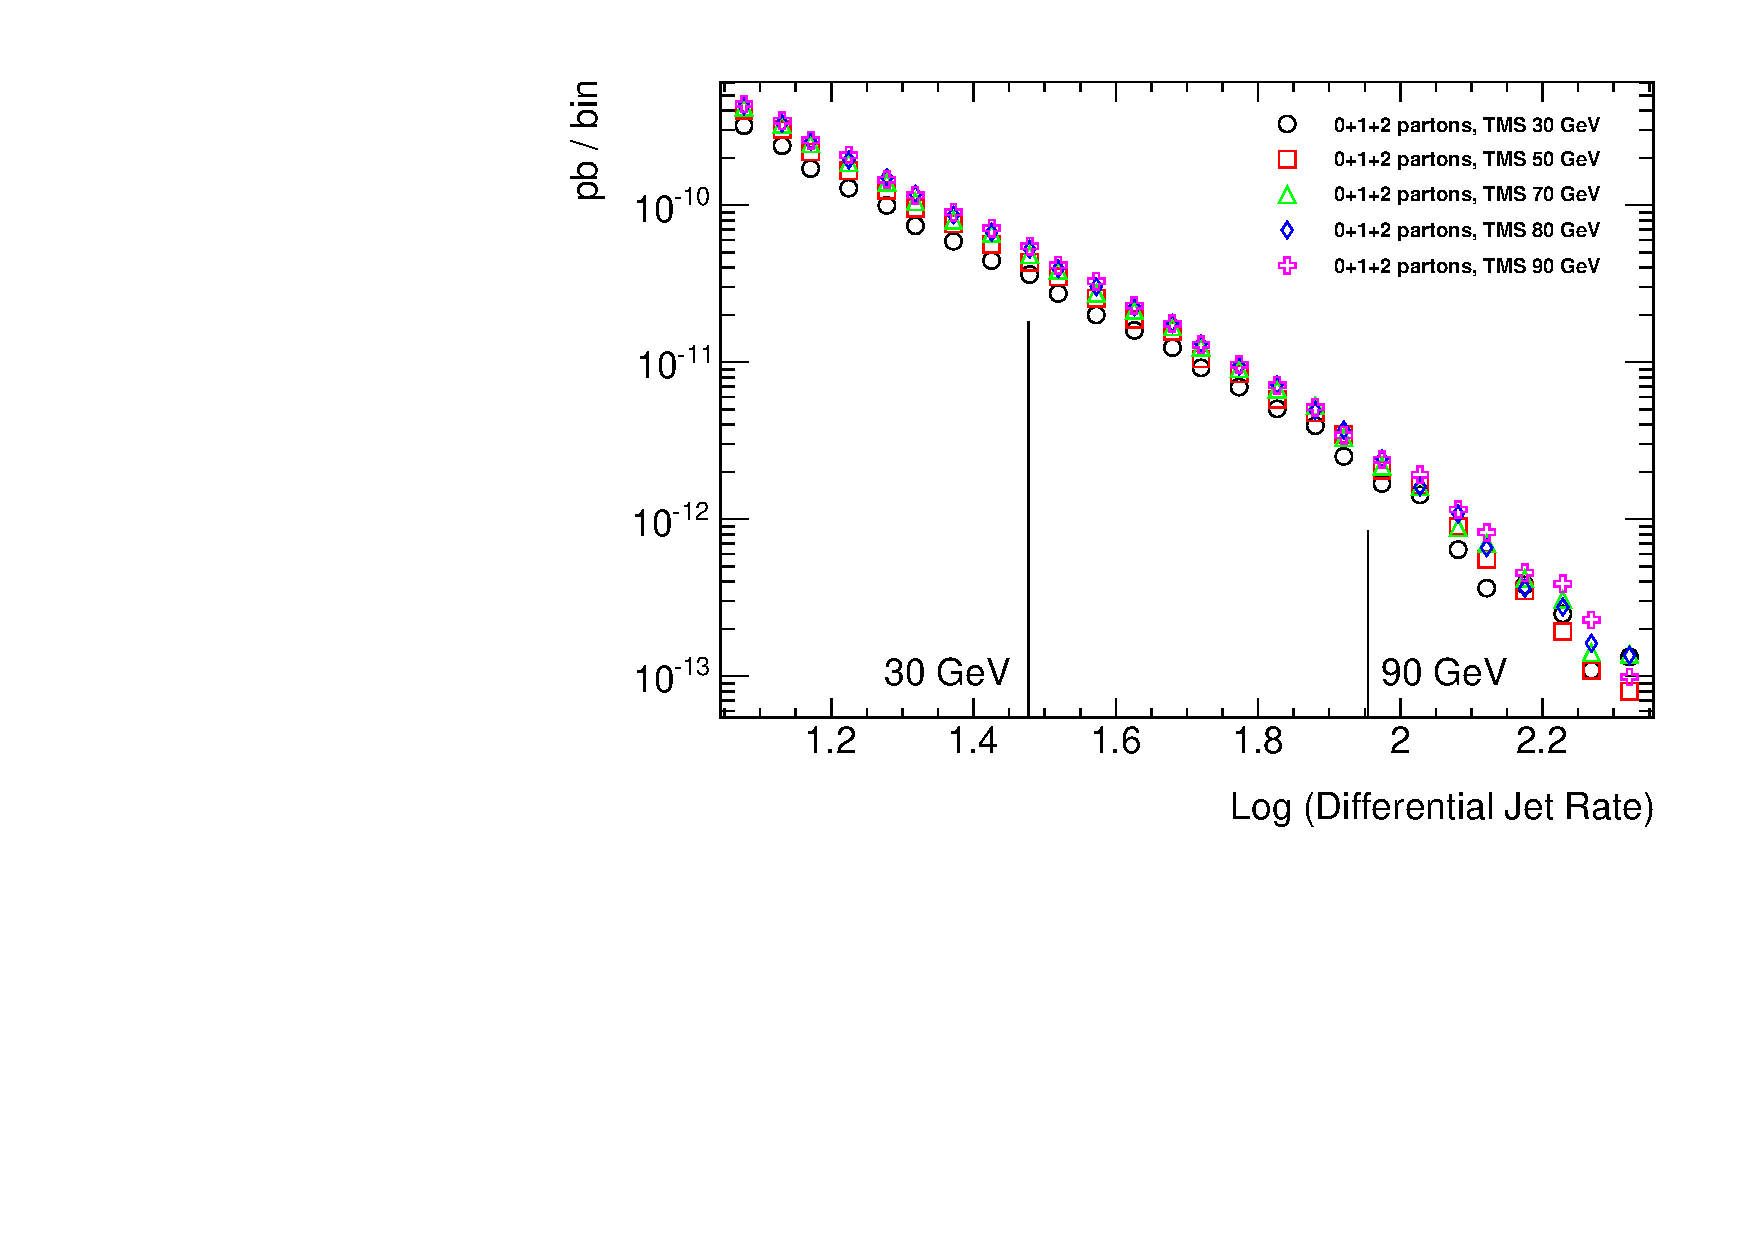
\includegraphics[width=0.48\linewidth]{figures/monojet_appendix/window_plot_4.pdf}
	}
  \caption{Jet differential rates distributions for EFT D5 sample with CKKW matching scale at 30, 50, 70, 80 and 90 GeV. 0-, 1- and 2-parton emission cases are generated separatedly and the total merged contribution is shown. A closer look is shown around the matching scale.}
  \label{fig:CKKW_D5_zoom}
\end{figure}


The MC distributions for the missing transverse energy and transverse momenta for the leading and subleading jets are plotted in Fig.. For the mono-jet analysis, usually a missing transverse energy cut larger than 300 GeV is applied for offline selection, which makes the contribution of the 0-parton emission case negligible in the mono-jet analysis.

\begin{figure}[h!]
	\centering  
%	\subfloat[Missing transverse momentum]{%
    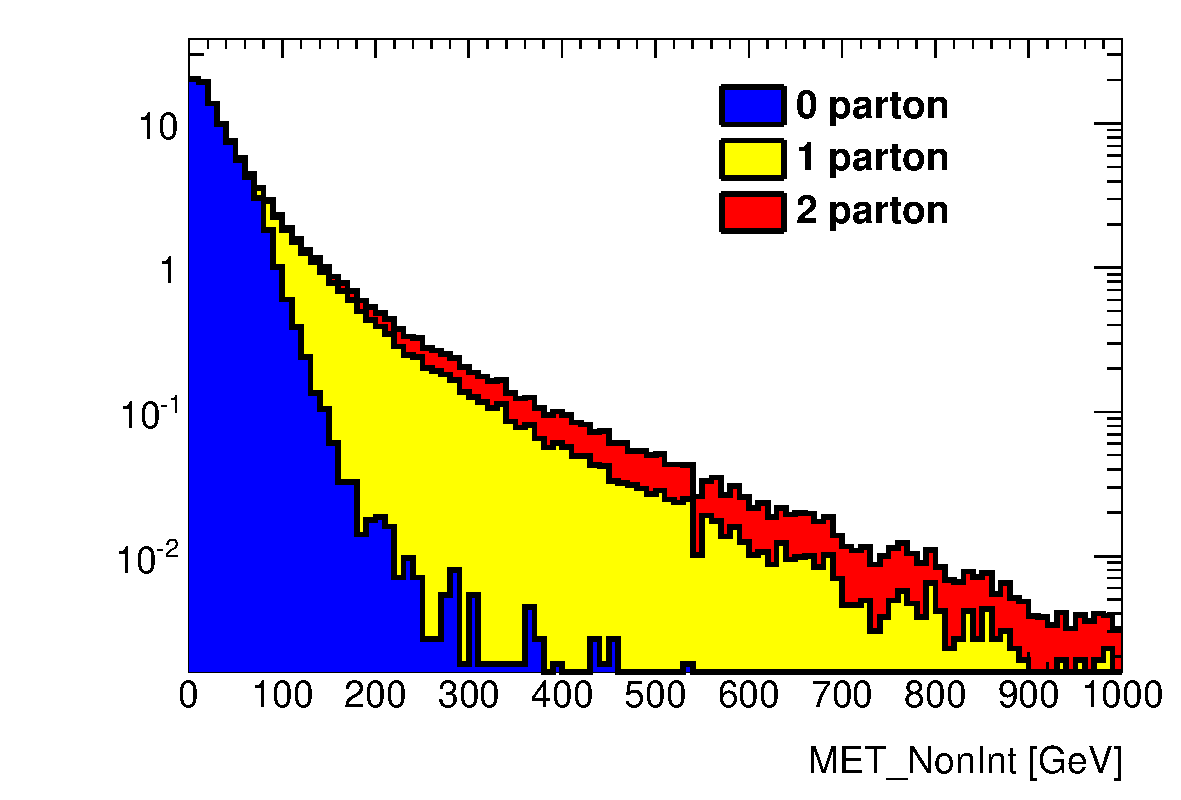
\includegraphics[width=0.8\linewidth]{figures/monojet_appendix/MET_matching80.pdf}
%	}
%	\hfill
%	\subfloat[Transverse momentum of leading jet]{%
%    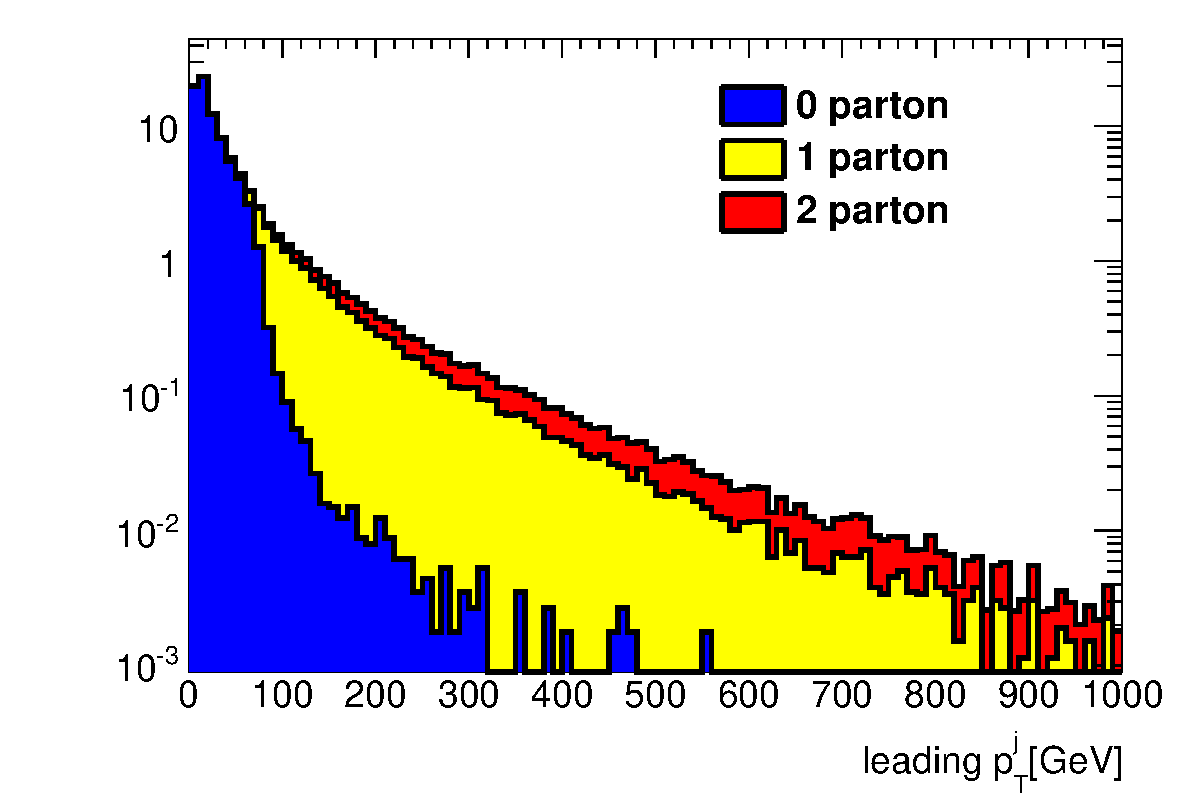
\includegraphics[width=0.48\linewidth]{figures/monojet_appendix/jet1pt_matching80.pdf}
%	}
%	\hfill
%	\subfloat[Transverse momentum of subleading jet]{%
%    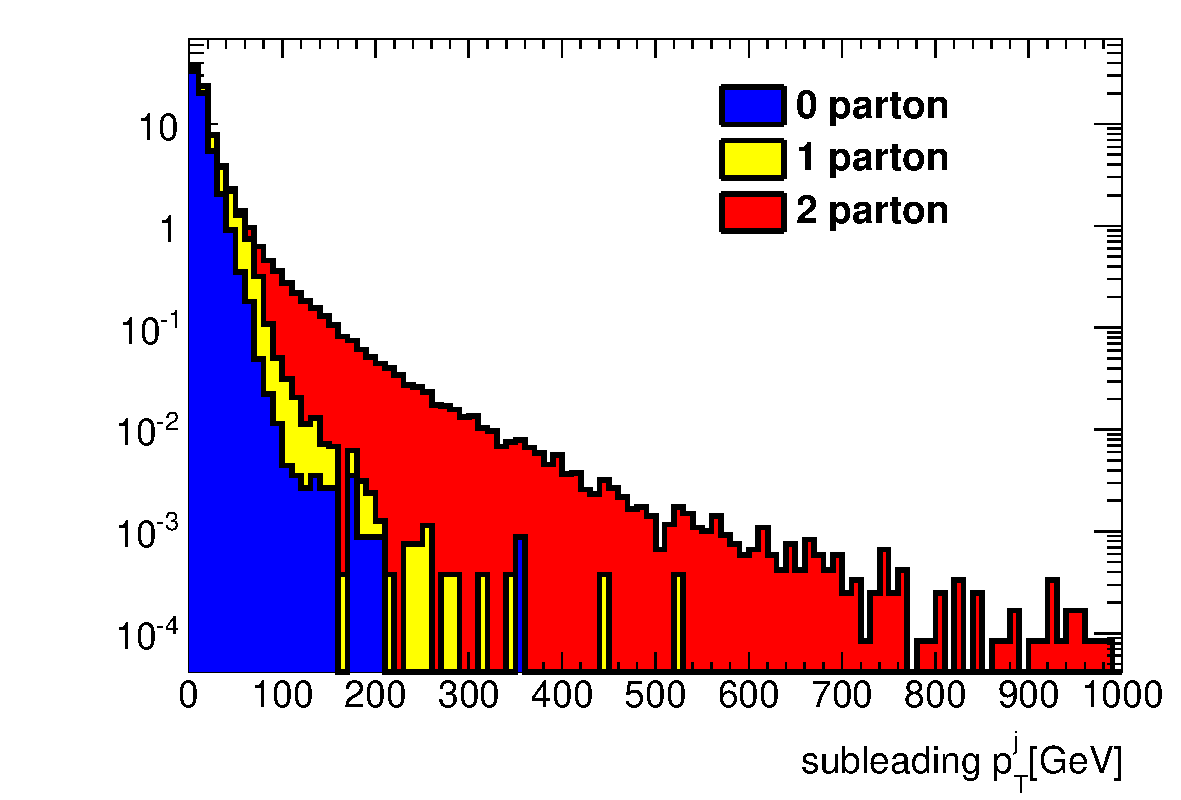
\includegraphics[width=0.48\linewidth]{figures/monojet_appendix/jet2pt_matching80.pdf}
%	}
%	\caption{Kinematics distributions for EFT D5 sample with CKKW matching scale at 80 GeV. 0-, 1- and 2-parton emission cases are generated separatedly and added together by cross sections. The 0-parton emission case has very limited contribution for missing transverse energy larger than 300 GeV region.}
	\caption{Missing transverse momentum distributions for EFT D5 sample with CKKW matching scale at 80 GeV. 0-, 1- and 2-parton emission cases are generated separatedly and added together by cross sections. The 0-parton emission case has very limited contribution for missing transverse energy larger than 300 GeV region.}
	\label{fig:Kine_D5_80}
\end{figure}


\section{Parton emission generation}
\label{sec:monojet_parton_emission}
In order to describe the signal kinematics correctly and save time in MC generation, the parton emissions will only be generated up to a certain numbers of parton and ignore the cases with more partons. The later ones usually have cross sections small enough and limited contribution in the interested kinematic regions.

It is found that the 3- or more-parton emission cases are negligible in our intersted regions, but the 2-parton emission case has significant contributions. The 0- and 1-parton emissions are out of discussion since they give the baseline signature in this analysis. The impacts of 2- and 3-parton emissions are quantified in this section.

Here the 0-, 1-, 2- and 3-parton emissions are generated separately and requested in matching step with \texttt{Merging:nJetMax=3} and scale at 80 GeV in Pythia8for 0+1+2+3 parton emission case, while \texttt{Merging:nJetMax=2} requested for 0+1+2 case and \texttt{Merging:nJetMax=1} requested for 0+1 case. The MET distribution is plotted in Fig.\ref{fig:RatioKine_D5}, while the jet multiplicity is shown in Fig.\ref{fig:RatioKine_D5_2}.

\begin{figure}[h!]
	\centering  
%	\subfloat[Missing transverse momentum]{%
	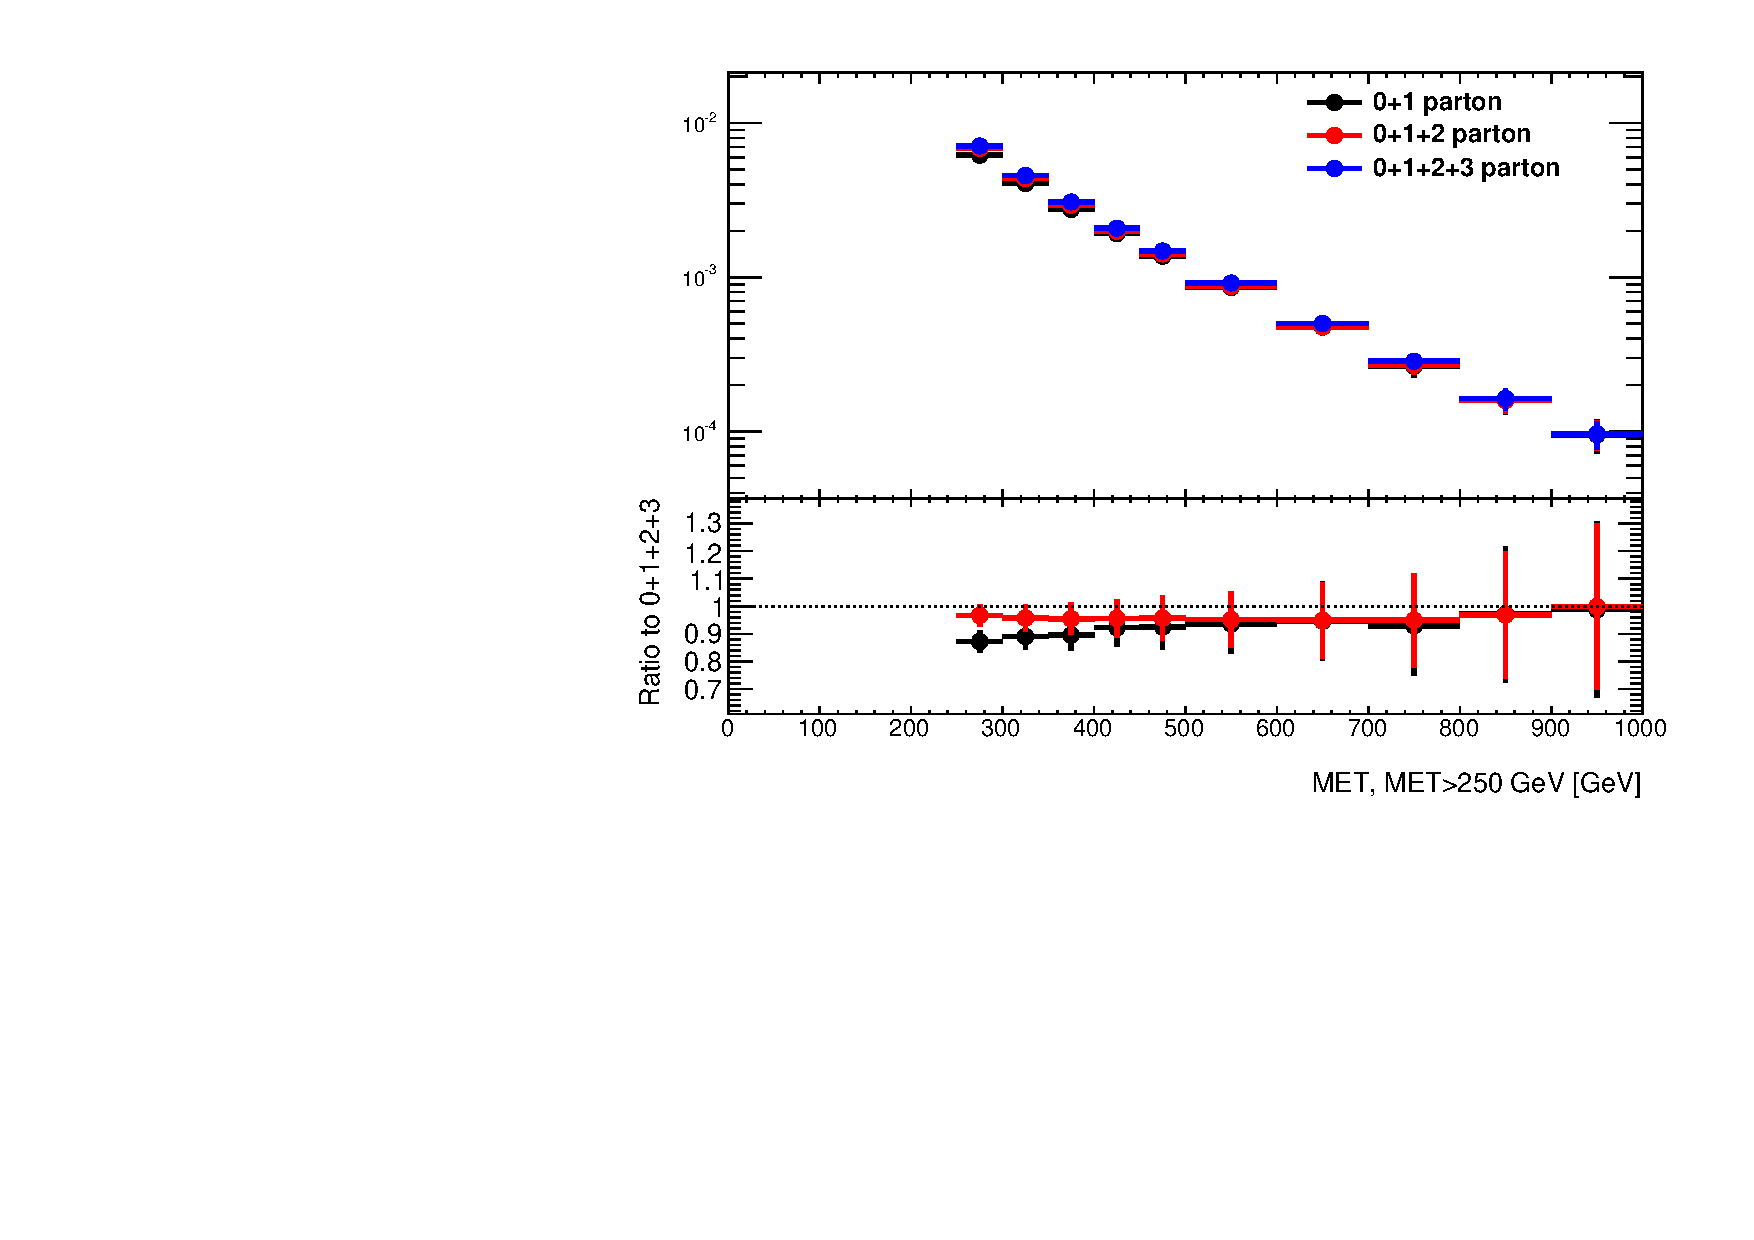
\includegraphics[width=0.8\linewidth]{figures/monojet_appendix/h_MET_MET250.pdf}
%	}
%	\hfill
%	\subfloat[Transverse momentum of leading jet]{%
%		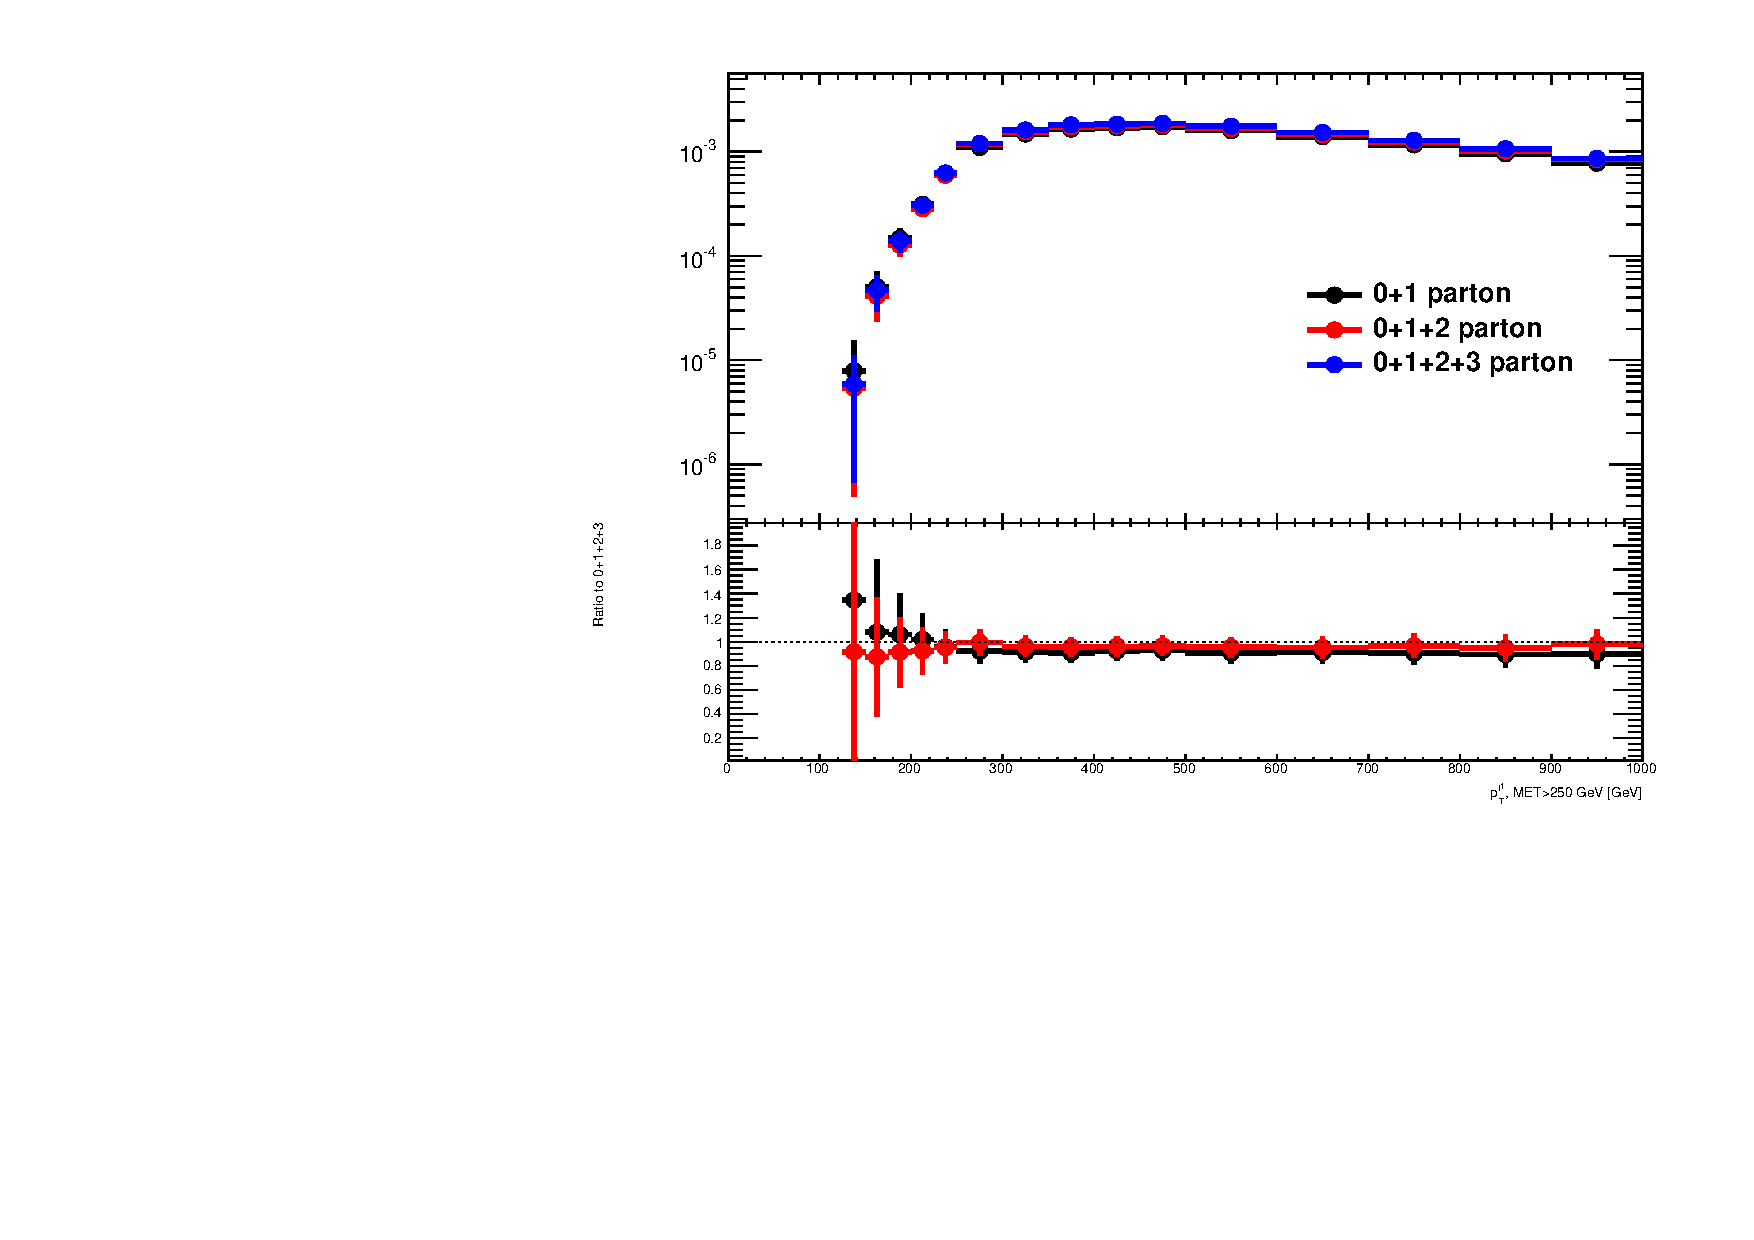
\includegraphics[width=0.48\linewidth]{figures/monojet_appendix/h_pt1_MET250.pdf}
%	}
%	\hfill
%	\subfloat[Transverse momentum of subleading jet]{%
%		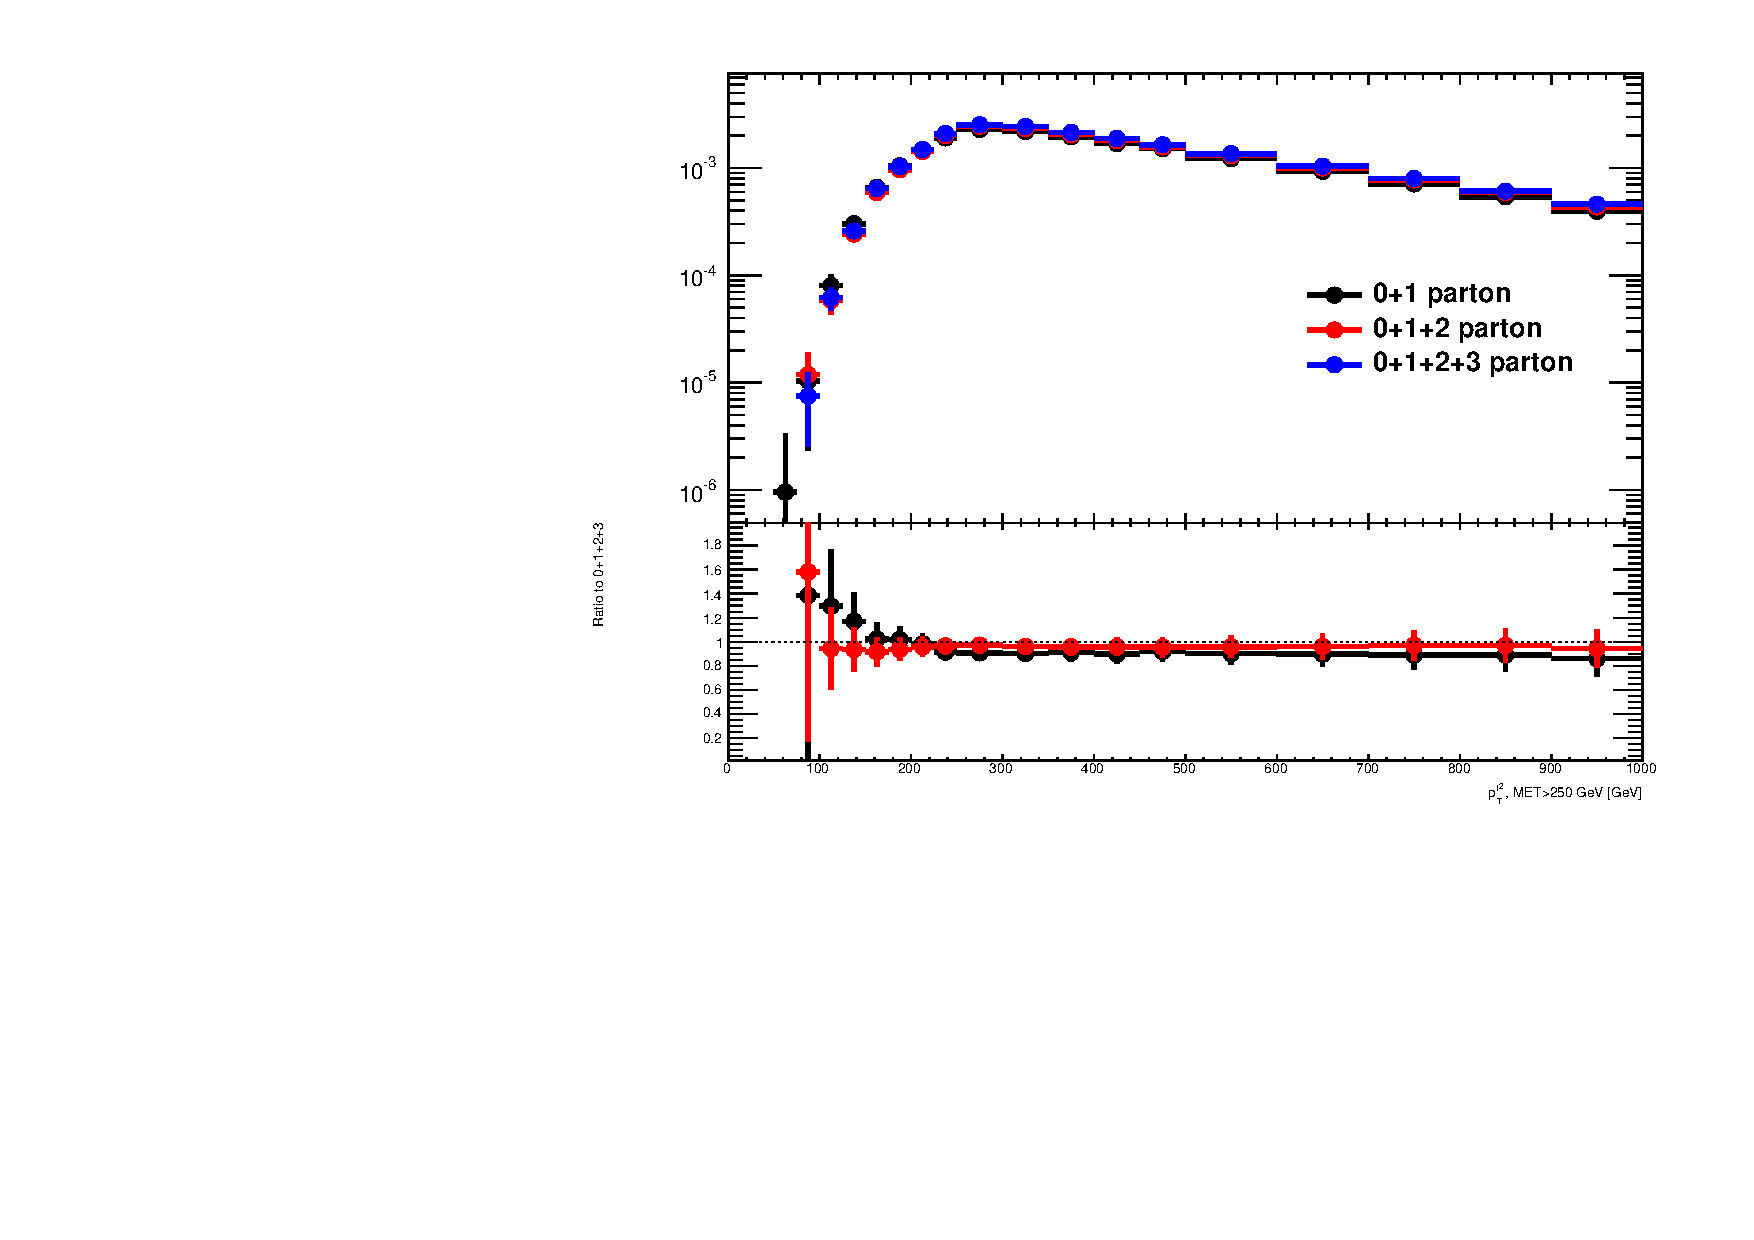
\includegraphics[width=0.48\linewidth]{figures/monojet_appendix/h_pt2_MET250.pdf}
%	}
%	\caption{Kinematics distributions for EFT D5 sample with CKKW matching scale at 80 GeV. 0-, 1-, 2- and 3-parton emission cases are generated separatedly and added together by cross sections.}
	\caption{Missing transverse momentum distributions for EFT D5 sample with CKKW matching scale at 80 GeV. 0-, 1-, 2- and 3-parton emission cases are generated separatedly and added together by cross sections.}
	\label{fig:RatioKine_D5}
\end{figure}


\begin{figure}[h!]
	\centering  
%	\subfloat[Jet multiplicity, leading jet $p_{T}>30$ GeV]{%
%    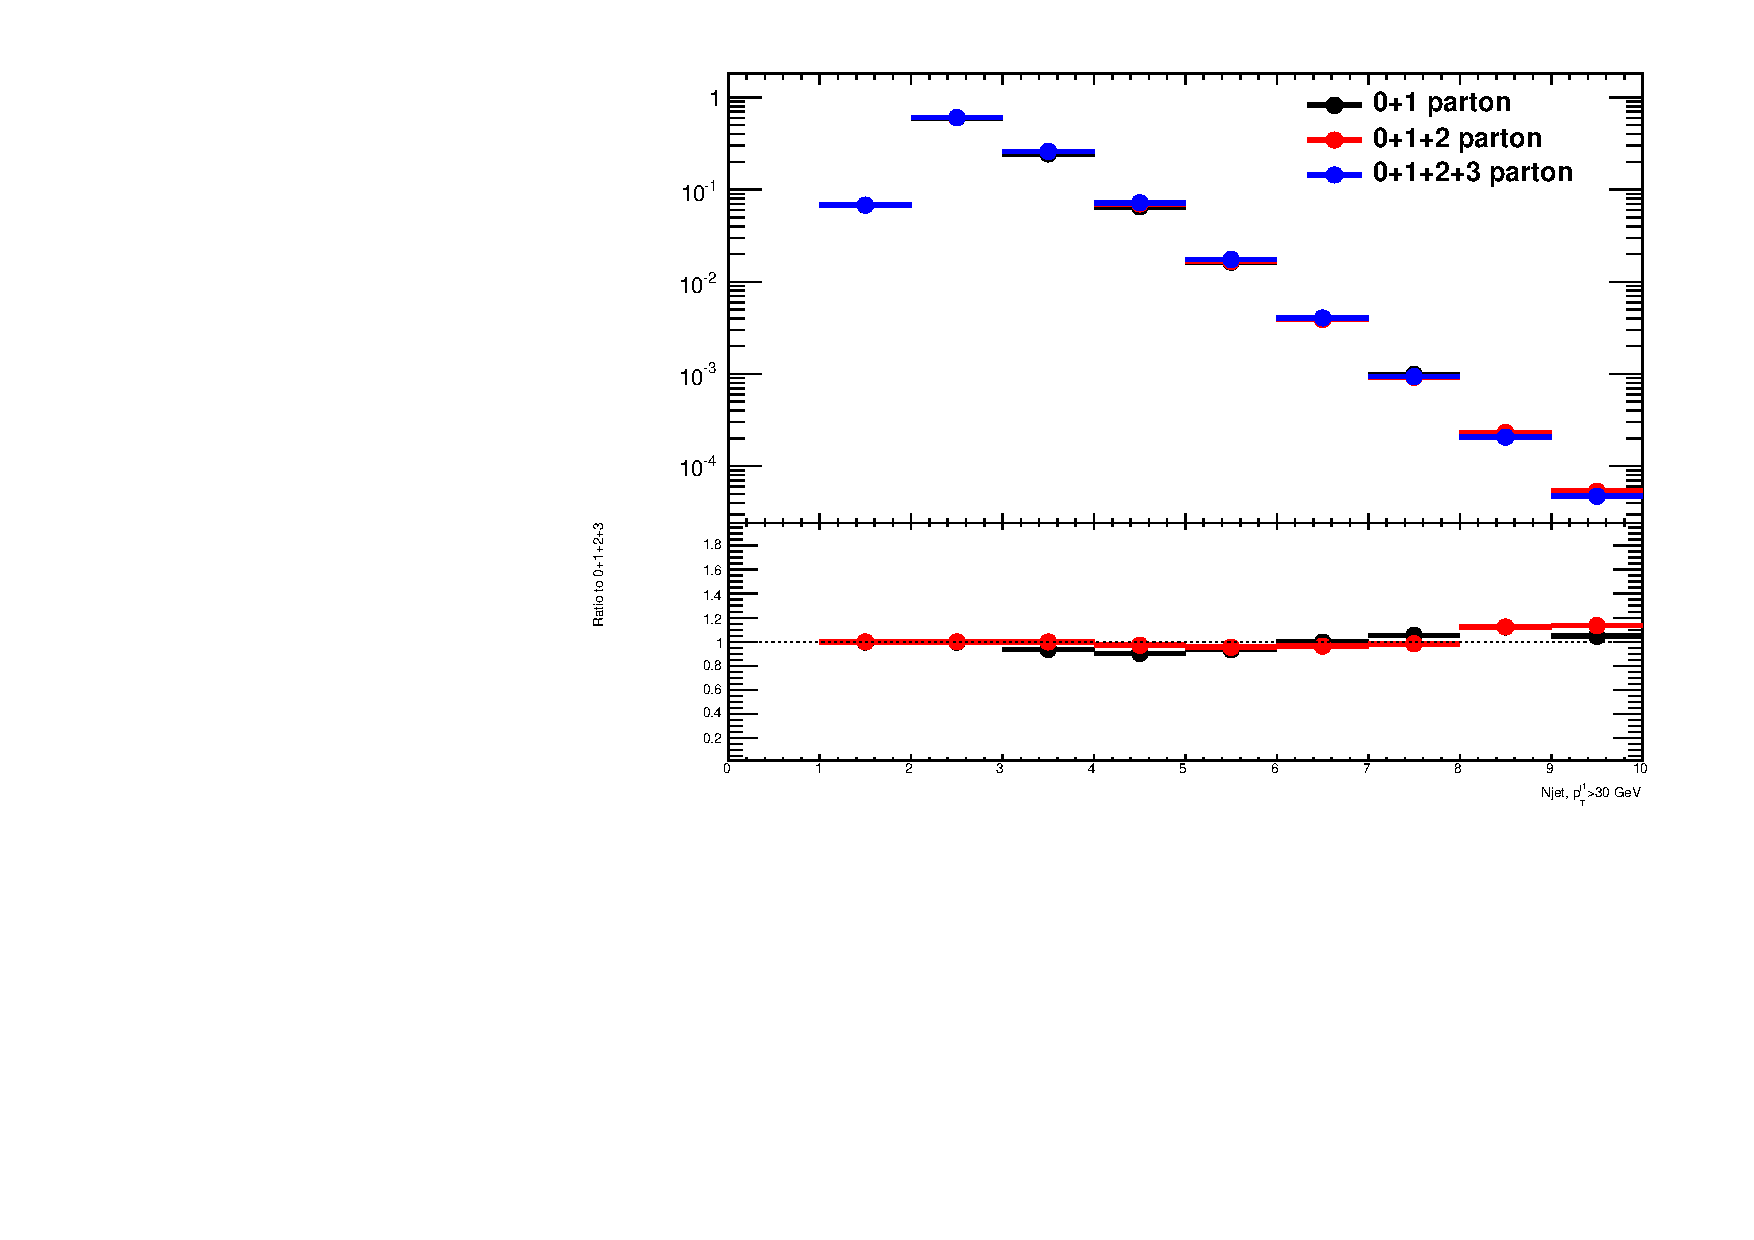
\includegraphics[width=0.48\linewidth]{figures/monojet_appendix/h_njet30.pdf}
%	}
%	\hfill
%	\subfloat[Jet multiplicity, leading jet $p_{T}>80$ GeV]{%
%    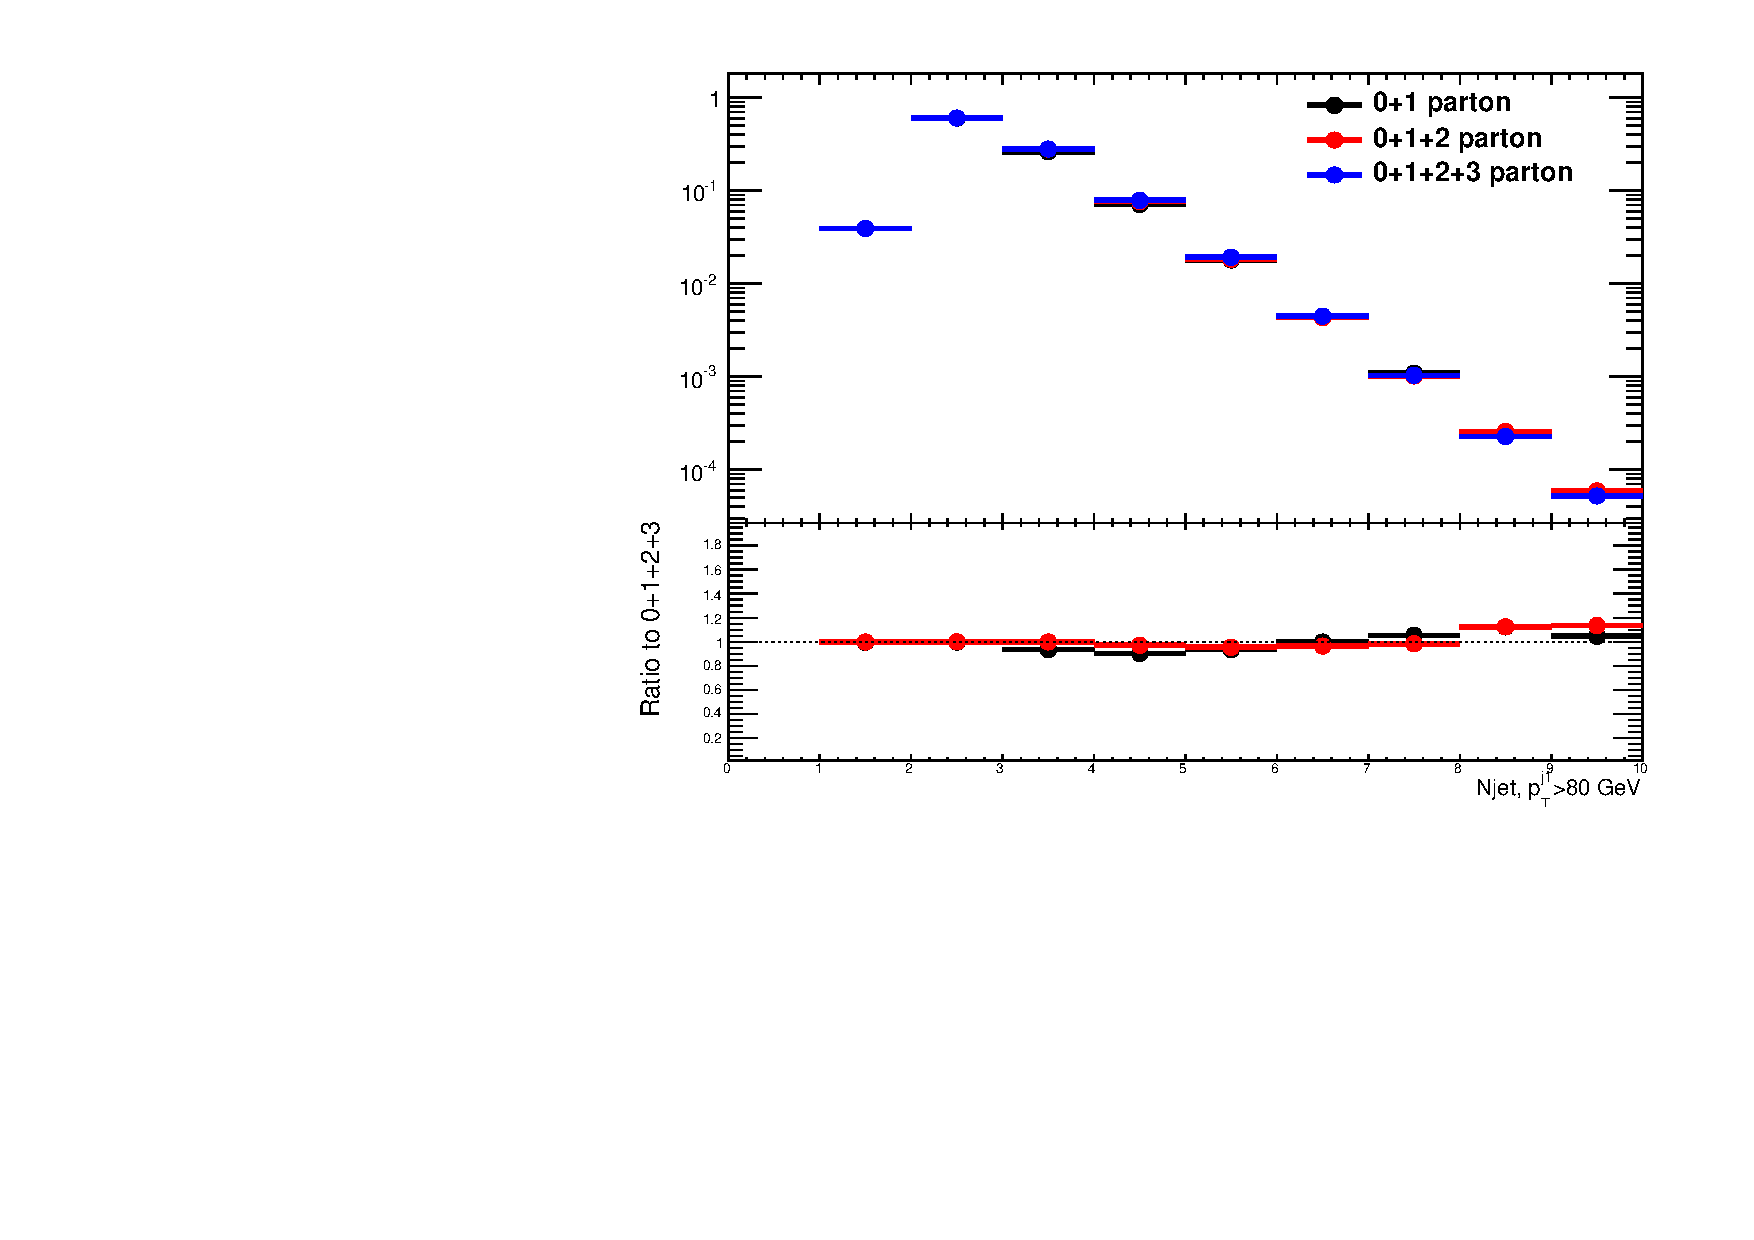
\includegraphics[width=0.48\linewidth]{figures/monojet_appendix/h_njet80.pdf}
%	}
%	\hfill
%	\subfloat[Jet multiplicity, leading jet $p_{T}>250$ GeV]{%
	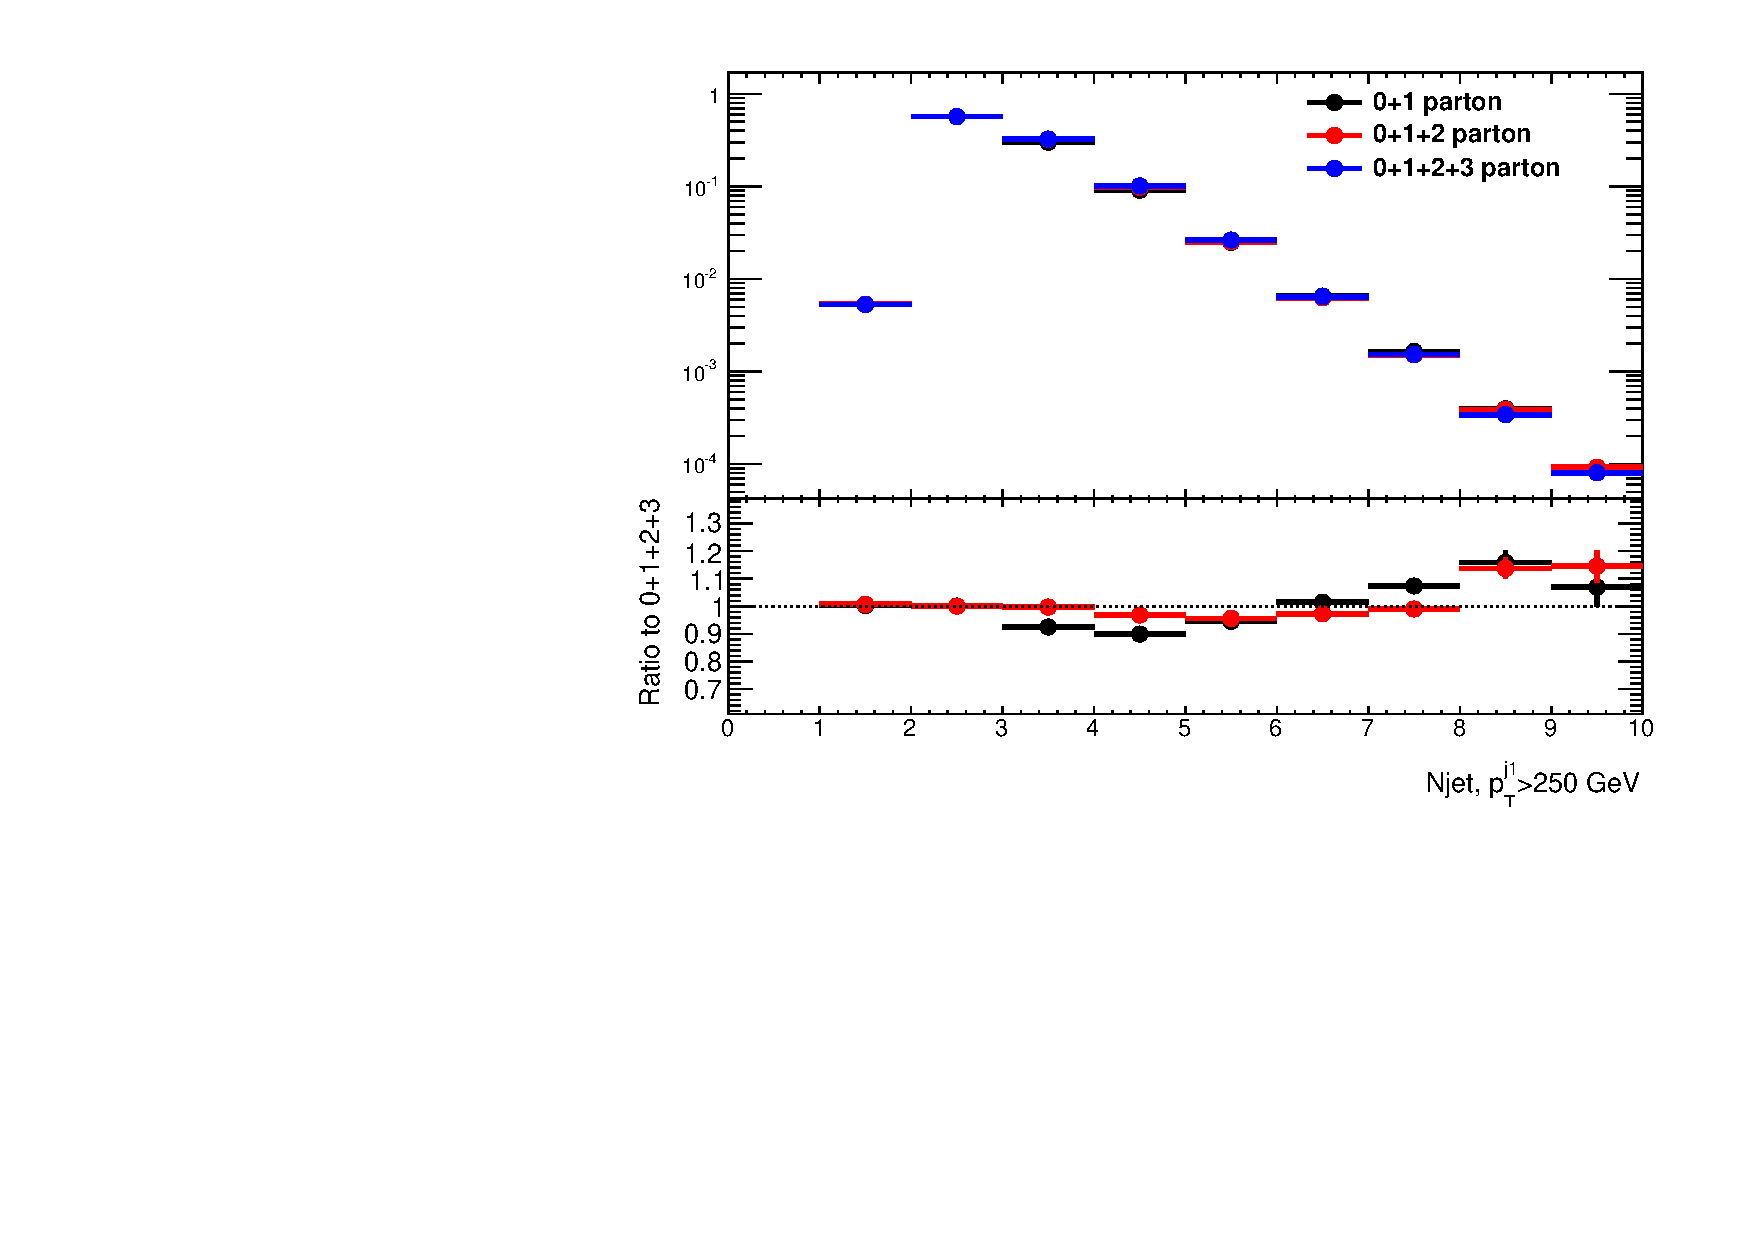
\includegraphics[width=0.8\linewidth]{figures/monojet_appendix/h_njet250.pdf}
%	}
%	\caption{Jet multiplicity distributions for EFT D5 sample with CKKW matching scale at 80 GeV. 0-, 1-, 2- and 3-parton emission cases are generated separatedly and added together by cross sections.}
	\caption{Jet multiplicity distribution for EFT D5 sample with CKKW matching scale at 80 GeV. 0-, 1-, 2- and 3-parton emission cases are generated separatedly and added together by cross sections.}
	\label{fig:RatioKine_D5_2}
\end{figure}

With the ATLAS run-I baseline cut (MET and leading jet $p_{T}$ larger than 250 GeV, less than 4 jets), the 0+1 parton emission has 17.4\% yield less compared to 0+1+2+3 parton emission, while the 0+1+2 has 2.2\% less. With MET$>$400 GeV, 0+1 parton emission has 16.8\% yield less and 0+1+2 parton emission has 2.4\% less compared to 0+1+2+3 parton emission. With MET$>$600 GeV, 0+1 parton emission has 16.5\% yield less and 0+1+2 parton emission has 2.9\% less compared to 0+1+2+3 parton emission. The same numbers hold if a sysmetric cut is added on leading jet transverse momentum.


\section{Model implementation for mono-Higgs models}

All three Higgs+MET models are generated at leading
order with MadGraph 2.2.2, using Pythia8 for the parton shower.
The MadGraph implementations of the scalar and vector models can be found on the Forum SVN 
repository~\cite{ForumSVN_EWMonoHiggs}, while the 2HDM model can be found
at this link~\cite{ForumSVN_EWMonoHiggs_2HDM}.

In all cases, it is recommended not to handle the $h$ decay through MadGraph as
it does not include the proper $h$ branching ratios, or, if using MadGraph, then the 
resulting cross section should be rescaled to match onto the correct branching ratio.

\newthought{Madgraph details for scalar mediator Higgs+MET model}

In this model, the contribution from the $gghS$ box is included through an effective 
Lagrangian evaluated in the large $m_t$ limit. 
This may overestimate the rates of the $h + \missET$ signal~\cite{Haisch:2012kf}, but a full evaluation
is left to future studies. 

\newthought{Madgraph details for 2HDM Higgs+MET model}
  
 The two couplings that can be changed in the Madgraph model follow the nomenclature below:
 \begin{itemize}
 	\item \texttt{Tb} - $\tan \beta$
 	\item \texttt{gz} - $g_z$, gauge coupling of $Z^\prime$ to quarks
 \end{itemize}
 The other couplings are not changed, including \texttt{gx} (the $A \bar \chi \chi$ coupling) which has little impact on the signal. 
 $\sin \alpha$ is fixed internally such that $\cos (\beta-\alpha) = 0$. 
 The width of the $Z^\prime$ and $A$ can be computed automatically within Madgraph. 
 The couplings here don't affect the signal kinematics, so they can be fixed to default values 
 and then the signal rates can be scaled appropriately. 
 
The nomenclature for the masses in the Madgraph model is:
 \begin{itemize}
 	\item \texttt{MZp} - PDG ID 32 - $Z^\prime$
 	\item \texttt{MA0} - PDG ID 28 - $A$
 	\item \texttt{MX} - PDG ID 1000022 - dark matter particle
 \end{itemize}
 
The other masses are unchanged and do not affect the result. 
 Both $Z^\prime \to hZ(\bar \nu \nu)$ and  $Z^\prime \to hA(\bar \chi \chi)$ contribute to the final state, scaling
 different with model parameters. We recommend to generate them separately, 
 and then add the two signal processes together weighted by cross sections.
 % These signals should be generated separately since they have different $\tan \beta, M_A$ dependence.  
 
